%!TEX root = ../phd-thesis-lei-ma.tex

\chapter{\label{chap:matter}Neutrino Oscillations in Oscillatory Matter Profile}

In certain regions inside a star or a supernova where convection is prominent, the matter density varies rapidly as a function of distance~\cite{Muller2015, Couch2015}. The neutrino flavor evolution in such environments is qualitatively different than that in a smooth density profile~\cite{Krastev1989, Loreti1994,Akhmedov2000, Friedland2006,Kneller2010,Kneller2013,Patton2014}. For example, the flavor conversion of the neutrino is greatly enhanced if the matter density fluctuates with certain wave numbers. This is known as parametric resonance.

To understand this interesting phenonema I will first introduce the background matter basis where the equation of motion simplifies. After demonstrating the simplest example of the parametric resonance in the presence of a sinusoidal matter profile with the Rabi formula, I will explain the interference effect when there exist multiple Fourier modes in the matter profile. Then I will show how to use the Jacobi-Anger expansion to decompose an arbitrary matter profile into a infinite sum of Fourier modes and how to apply the Rabi formula in these scenarios.

% In Sec.~\ref{sec:jacobi} we discuss the technique of decomposing the neutrino flavor conversions into summation of Rabi oscillations, by applying a specific unitary transformation and the Jacobi-Anger expansion. As the system is exactly decomposed into multiple Rabi oscillations, we can interpret neutrino flavor oscillations in any matter density fluctuations, in principle. As an example, we solve the neutrino flavor transitions in a castle wall matter profile, which contains infinite frequencies from the aspect of Fourier series. Finally I will discuss an algorithm to select the Fourier modes of a matter profile that have the largest impact on the flavor conversion of the neutrino.



% \section{\label{chap:basics-section:astro}Stars as Neutrino Factories}


% In the following sections of this chapter, I will discuss neutrino oscillations in the Sun as well as in supernovae. Solar neutrinos go through a region with smoothly decreasing matter density while supernova neutrinos go through a region with turbulent matter background~\cite{Friedland2006,Borriello2014}. Neutrino oscillations within the supernova is quite different from neutrino oscillations in the Sun.




\section{\label{chap:matter-sec:background}Background Matter Basis}

% \fbox{TODO: Explain why two flavor} didn't add this because the three flavor is really very different.

% I will write down the equation of motion for neutrinos prograting through a general matter profile $\lambda(r)$ where $r$ is the trajectory of neutrinos. The Hamiltonian of neutrino oscillations is Eqn.~\ref{chap:basics-sec:msw-eqn:hamiltonian-matter-effect}. The dynamics of neutrino flavor conversion is determined by the Schr\"{o}dinger equation:
% \begin{equation*}
%     \mathrm i\frac{\mathrm d}{\mathrm d r}\Psi(r) = \frac{1}{2} \left(
%     (- \omega_{\mathrm{v}}\cos 2\theta_{\mathrm{v}} + \lambda(r) ) \sigma_3 + \omega_{\mathrm{v}}\sin 2\theta_{\mathrm{v}} \sigma_1
%     \right)
%     \Psi(r),
% \end{equation*}
% where $\Psi(r)$ is the wave function in flavor basis. For the two flavor scenario, the wave function is written as
% \begin{equation}
% 	 \Psi(r) = \begin{pmatrix}
%     \psi_{\ee} \\
%     \psi_{\xx}
% 	\end{pmatrix},
% \end{equation}
% where $\psi_{\ee}$ and $\psi_{\xx}$ are the amplitudes for electron flavor and the other flavor ($\mu$ flavor or $\tau$ flavor) respectively.

For a uniform matter density $\lambda(r) = \lambda_0$, one can define a matter basis in which the Hamiltonian is diagonalized:
\begin{equation}
\mathsf H^{(\mm)}  = \mathsf U^\dagger \mathsf H^{(\ff)} \mathsf U = -\frac{\omega_\mm}{2} \sigma_3,
\end{equation}
where
\begin{equation}
\mathsf U = \begin{pmatrix}
\cos \theta_\mm & \sin \theta_\mm \\
\sin\theta_\mm & \cos \theta_\mm
\end{pmatrix}
\end{equation}
with
\begin{equation*}
\theta_{\mathrm{m}}= \frac{1}{2} \arctan\left(
\frac{\sin 2\theta_{\mathrm v}}{ \cos 2\theta_{\mathrm v} - \lambda_0/\omega_{\mathrm v} } \right),
\label{chap:matter-sec:background-eqn:thetam}
\end{equation*}
and
\begin{equation}
\omega_{\mathrm{m}} = \omega_{\mathrm{v}} \sqrt{ ( \lambda_0/\omega_{\mathrm{v}} - \cos (2\theta_{\mathrm{v}}) )^2 + \sin^2(2\theta_{\mathrm{v}}) }
\label{chap:matter-sec:background-eqn:omegam}
\end{equation}
is the neutrino oscillations frequency in matter.

In the rest of the chaper, I will consider profiles of the form
\begin{equation}
    \lambda(r) = \lambda_0 + \delta \lambda(r),
    \label{eq-general-matter-profile}
\end{equation}
where $\delta \lambda(r)$ describes the fluctuation of the matter density. I will use the background matter basis defined by Eqn.~\ref{chap:matter-sec:background-eqn:thetam} and Eqn.~\ref{chap:matter-sec:background-eqn:omegam}. In this basis, the Hamiltonian reads
\begin{equation}
    \mathsf H^{(\mathrm{m})} = -\frac{\omega_\mm}{2} \sigma_3 + \frac{1}{2} \delta\lambda(r) \cos 2\theta_{\mathrm m} \sigma_3
     - \frac{1}{2} \delta\lambda(r) \sin 2\theta_{\mathrm m} \sigma_1.
    \label{eq-hamiltonian-bg-matter-basis-general}
\end{equation}

In the background matter basis, the wave function describes the amplitudes of different eigenstates defined when there is only background matter density $\lambda_0$. Given the transition probability between the these eigenstates, it is trivial to calculate the flavor conversion. Since I'll concentrate on the flavor conversion due to the matter fluctuations, I'll only discuss the transition between mass states in the background matter basis.

All the numerical examples in this chapter are calculated with $\sin^2(2\theta_{\mathrm v}) = 0.093$ and $\omega_{\vv} = 3.75\times 10^{-17}\mathrm{MeV}^2$.
%$\delta m^2 = 2.6\times 10^{-3}\mathrm{eV}^2$.



%%%%%%%%%%%%%%%%%%%%%%%%%%%%%%%%%%%%%%%%%%%%%%%%%%%%
%% Single frequency
%%%%%%%%%%%%%%%%%%%%%%%%%%%%%%%%%%%%%%%%%%%%%%%%%%%%



\section{\label{chap:matter-sec:single}Single Frequency Matter Profile and Rabi oscillations}%


In this section I will present a simple picture to explain neutrino parametric resonance in matter by utilizing the theory of Rabi oscillations. Rabi oscillations have been well studied in quantum optics~\cite{Boyd2008}. It describes the transition between different quantum states due to an oscillatory external driving field, where maximum transition or resonance happens when the frequency of external driving field equals the energy gap. In this section, I will first derive the Rabi oscillation transition probabilities using neutrino flavor isospin method introduced in Ref.~\cite{Duan2006a}. Then I will apply the results of Rabi oscillations to neutrino oscillations in single frequency matter profile.


\subsection{\label{chap:app-sec:rabi-oscillations}Rabi Oscillations}

\begin{figure}[htbp]
    \centering
    % 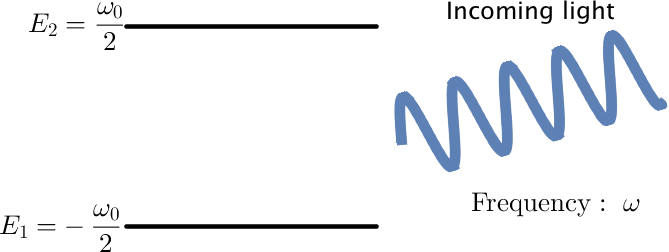
\includegraphics[width=0.6\textwidth]{chapters/assets/app/rabi-diagram.png}
    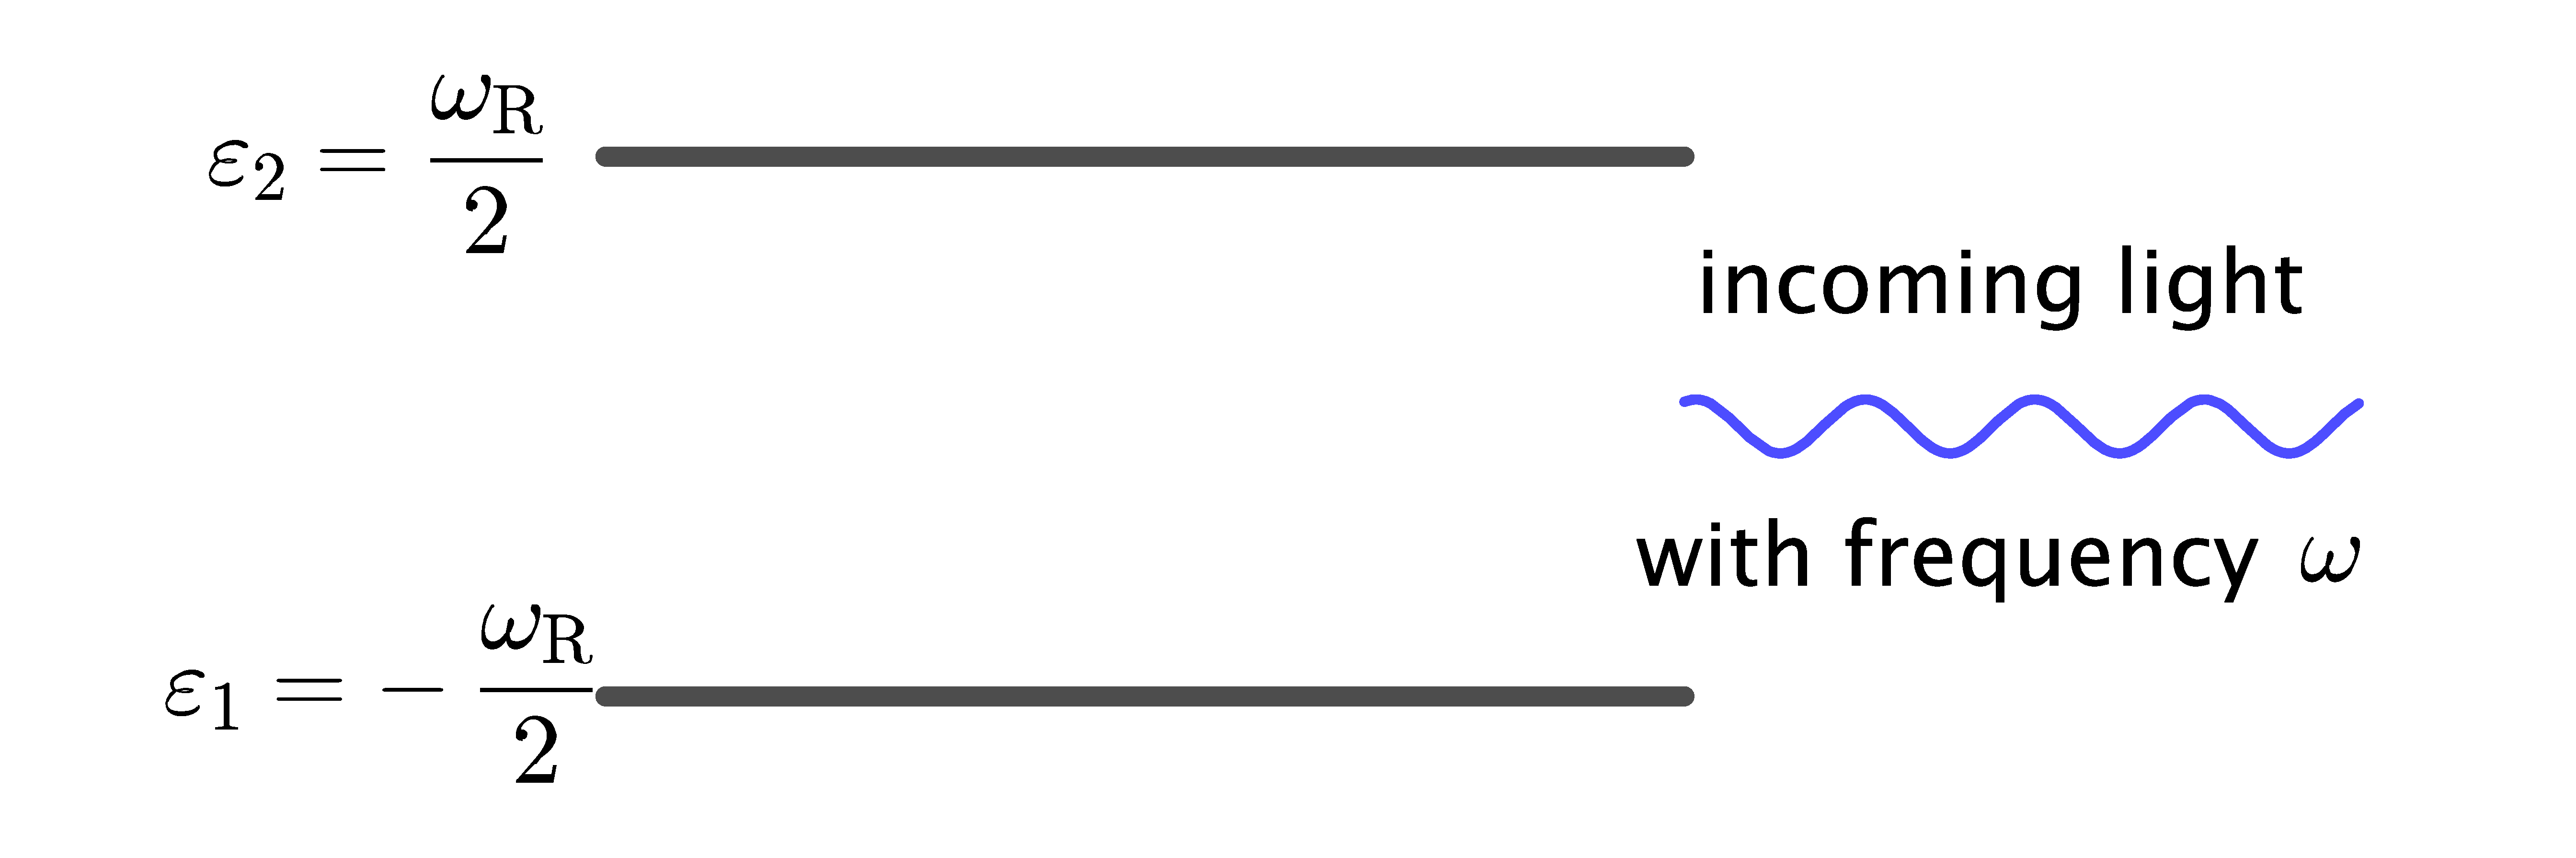
\includegraphics[width=0.7\textwidth]{chapters/assets/matter/rabi-illustrative-diagram}
    \caption{Schematic illustration of Rabi oscillations system. The two level system has two energy states at $\varepsilon_1=-\frac{\omega_\RR}{2}$ and $\varepsilon_2=\frac{\omega_\RR}{2}$. Resonance happens when the freuquency of the driving field $\omega$ equals the energy gap $\omega_\RR$, i.e., $\omega = \omega_\RR$.}
    \label{chap:app-sec:rabi-oscillations-fig:rabi-diagram}
\end{figure}

An example of Rabi oscillations is a two-level quantum system with energy gap $\delta\varepsilon = \omega_{\RR}$ and light of frequency $\omega$ shining on the two-level system (see Fig.~\ref{chap:app-sec:rabi-oscillations-fig:rabi-diagram}).
The Hamiltonian for Rabi oscillation is
\begin{equation}
    \mathsf H_{\RR} = -\frac{\omega_{\RR}}{2}\sigma_3 - \frac{A_{\RR} }{2}  \left( \cos(k_{\RR} t +\phi_{\RR})\sigma_1  - \sin(k_{\RR} t +\phi_{\RR}) \sigma_2\right),
    \label{rabi-oscillation-single-perturbation}
\end{equation}
in which $\omega_{\RR}$ serves as the energy split of the two level system, while $A_{\RR}$ and $k_{\mathrm{R}}$ are the strength and frequency of the driving field, respectively. The Hamiltonian $\mathsf H_\RR$ can be mapped into a vector using the flavor isospin picture:
\begin{equation*}
% H_{\mathrm R}
% = - \frac{\boldsymbol{\sigma}}{2} \cdot (\mathbf{H}_3 + \mathbf{H}_+ ) ,
\vec H_{\RR} = \vec H_3 + \vec H_+,
\end{equation*}
where
\begin{align}
    \vec{H}_3 = & \begin{pmatrix}
    0 \\ 0 \\ \omega_{\mathrm R}
    \end{pmatrix}, \\
    \vec{H}_+ = & \begin{pmatrix}
    A_{\mathrm{R}} \cos(k_{\mathrm{R}} t +\phi_{\mathrm{R}}) \\
    - A_{\mathrm{R}} \sin(k_{\mathrm{R}} t +\phi_{\mathrm{R}}) \\
    0
    \end{pmatrix}.
    \label{chap:app-sec:rabi-eqn:h3-and-hplus}
\end{align}
The above two vectors are mapped into a Cartesian coordinate system similar to the flavor isospin space~\footnote{ The phase $\phi_{\mathrm{R}}$ of the driving potential in Eqn.~\ref{rabi-oscillation-single-perturbation} has no effect on the transition probability since it only determines the initial phase of driving Hamiltonian vector $\vec{H}_+$. The oscillation amplitude is not affected by $\phi_\RR$ at all.}. The vector $\vec{H}_3$ is the vector aligned with the third axis, $\vec{H}_+$ is a rotating vectors in a plane perpendicular to $\vec{H}_3$ (see Fig.~\ref{chap:app-sec:rabi-fig:rabi-static-frame}). The wave function $\Psi=(\psi_1,\psi_2)^{\mathrm{T}}$ is also used to define the state vector $\vec{s}$
\begin{align}
    \vec{s} =& \Psi^\dagger \frac{\vec{\sigma}}{2}\Psi \\
    =& \frac{1}{2}\begin{pmatrix}
    2\,\mathrm{Re}\,(\psi_1^* \psi_2) \\
    2\,\mathrm{Im}\,(\psi_1^*\psi_2) \\
    \lvert \psi_1 \rvert^2 - \lvert \psi_2 \rvert^2
    \end{pmatrix}
\end{align}



\begin{figure}[htbp]
	\centering
	\begin{subfigure}[t]{0.5\textwidth}
		\centering
		\includegraphics[width=0.8\textwidth]{chapters/assets/matter/rabi-isospin-static-frame}
		\caption{Static frame}\label{chap:app-sec:rabi-fig:rabi-static-frame}
	\end{subfigure}%
	% \quad
	\begin{subfigure}[t]{0.5\textwidth}
		\centering
		\includegraphics[width=0.85\textwidth]{chapters/assets/matter/rabi-isospin-rotating-frame}
		\caption{Corotatting frame}\label{chap:app-sec:rabi-fig:rabi-rotating-frame}
	\end{subfigure}
	\caption{
  Rabi oscillations in different frames. The vectors $\vec H_3$ and $\vec H_+$ are defined in Eqn.~\ref{chap:app-sec:rabi-eqn:h3-and-hplus}. The red dashed vectors are the flavor isospins. The black solid vectors are the vectors that stand for Hamiltonians.
  }\label{chap:app-sec:rabi-fig:rabi-frames}
\end{figure}


The third component of $\vec{s}$, which is denoted as $s_3$, is within range $[-1/2,1/2]$. The two limits, $s_3=-1/2$ and $s_3=1/2$ stand for the two-level system in high energy state and low energy state respectively. If the two-level system has equal probabilities to be on high energy state and low energy state, I have $s_3=0$. The equation of motion is given by Eqn.~\ref{chap:basics-sec:flavor-isospin-pic-eqn:eom-precession}. In this example, the total ``Hamiltonian vector" $\vec H$ is not static since it has a rotating component $\vec H_+$. I need a better frame to understand the evolution of the state vector $\vec s$.

% \begin{figure}[htbp]
%         \centering
%         \includegraphics[width=\columnwidth, trim={20cm 10cm 50cm 10cm},clip]{chapters/assets/rabi/rabi-isospin-rotating-frame}
%     \caption{Rabi oscillations in corotating frame. The red dashed vector is the flavor isospin, while the black solid vectors are the vectors of Hamiltonian. The flavor isospin vector is precessing around vector of total Hamiltonian $\vec{H}_3+\vec{H}_+$.}
%     \label{fig-rabi-isospin-rotating-frame}
% \end{figure}



A more convenient frame is the frame that corotates with $\vec{H}_+$, which is described in Fig.~\ref{chap:app-sec:rabi-fig:rabi-rotating-frame}. The Hamiltonian in this frame is
\begin{equation}
\frac{\mathrm d}{\mathrm d t } \vec{s} = \vec{s} \times (\vec{H}'_3 + \vec{H}_+),
\end{equation}
where
\begin{equation}
\vec{H}'_3 = \begin{pmatrix}
    0 \\ 0 \\  \omega_{\mathrm{R}} - k_{\mathrm R}
  \end{pmatrix}, \qquad \vec{H}'_+ = \begin{pmatrix}
    A_{\mathrm{R}} \\ 0 \\  0
    \end{pmatrix}.
\end{equation}
The state vector $\vec{s}$ precesses around the static vector $\vec{H}'_3 + \vec{H}'_+$ in this corotatting frame with a frequency $\Omega_{\mathrm R} = \sqrt{ \lvert A_{\mathrm{R}}\rvert^2 + (k_{\mathrm{R}} - \omega_{\mathrm R})^2 }$. An analysis by projecting the state vector $\vec{s}$ on to the vertical axis shows that
\begin{equation}
s_3 = \frac{1}{2} - \frac{\lvert A_{\mathrm R}\rvert ^2}{\Omega_{\mathrm R}^2}\sin^2\left(\frac{\Omega_{\mathrm R}}{2} t\right).
\end{equation}
Such a system has an analytical transition probability from low energy state to high energy state, as know as the Rabi formula,
\begin{equation}
    P(t) = \frac{1}{2}(1- 2 s_3(t))= \frac{\left \lvert A_{\mathrm{R}} \right \rvert ^2}{ \Omega_{\mathrm R}^2 } \sin^2 \left( \frac{\Omega_{\mathrm R}}{2} t \right),
    \label{app:rabi-system-transition-probability}
\end{equation}
where
\begin{equation}
\Omega_{\mathrm R} = \sqrt{ \lvert A_{\mathrm{R}}\rvert^2 + (k_{\mathrm{R}} - \omega_{\mathrm R})^2 }
\label{app:rabi-frequency}
\end{equation} is known as the Rabi frequency. The amplitude $A_\RR$ is the dominate factor of oscillation frequency when the rabi oscillation is close to resonance. Fig.~\ref{app-fig:rabi-examples} shows two examples of the transition probabilities of Rabi oscillations.

\begin{figure}[htbp]
    \centering
    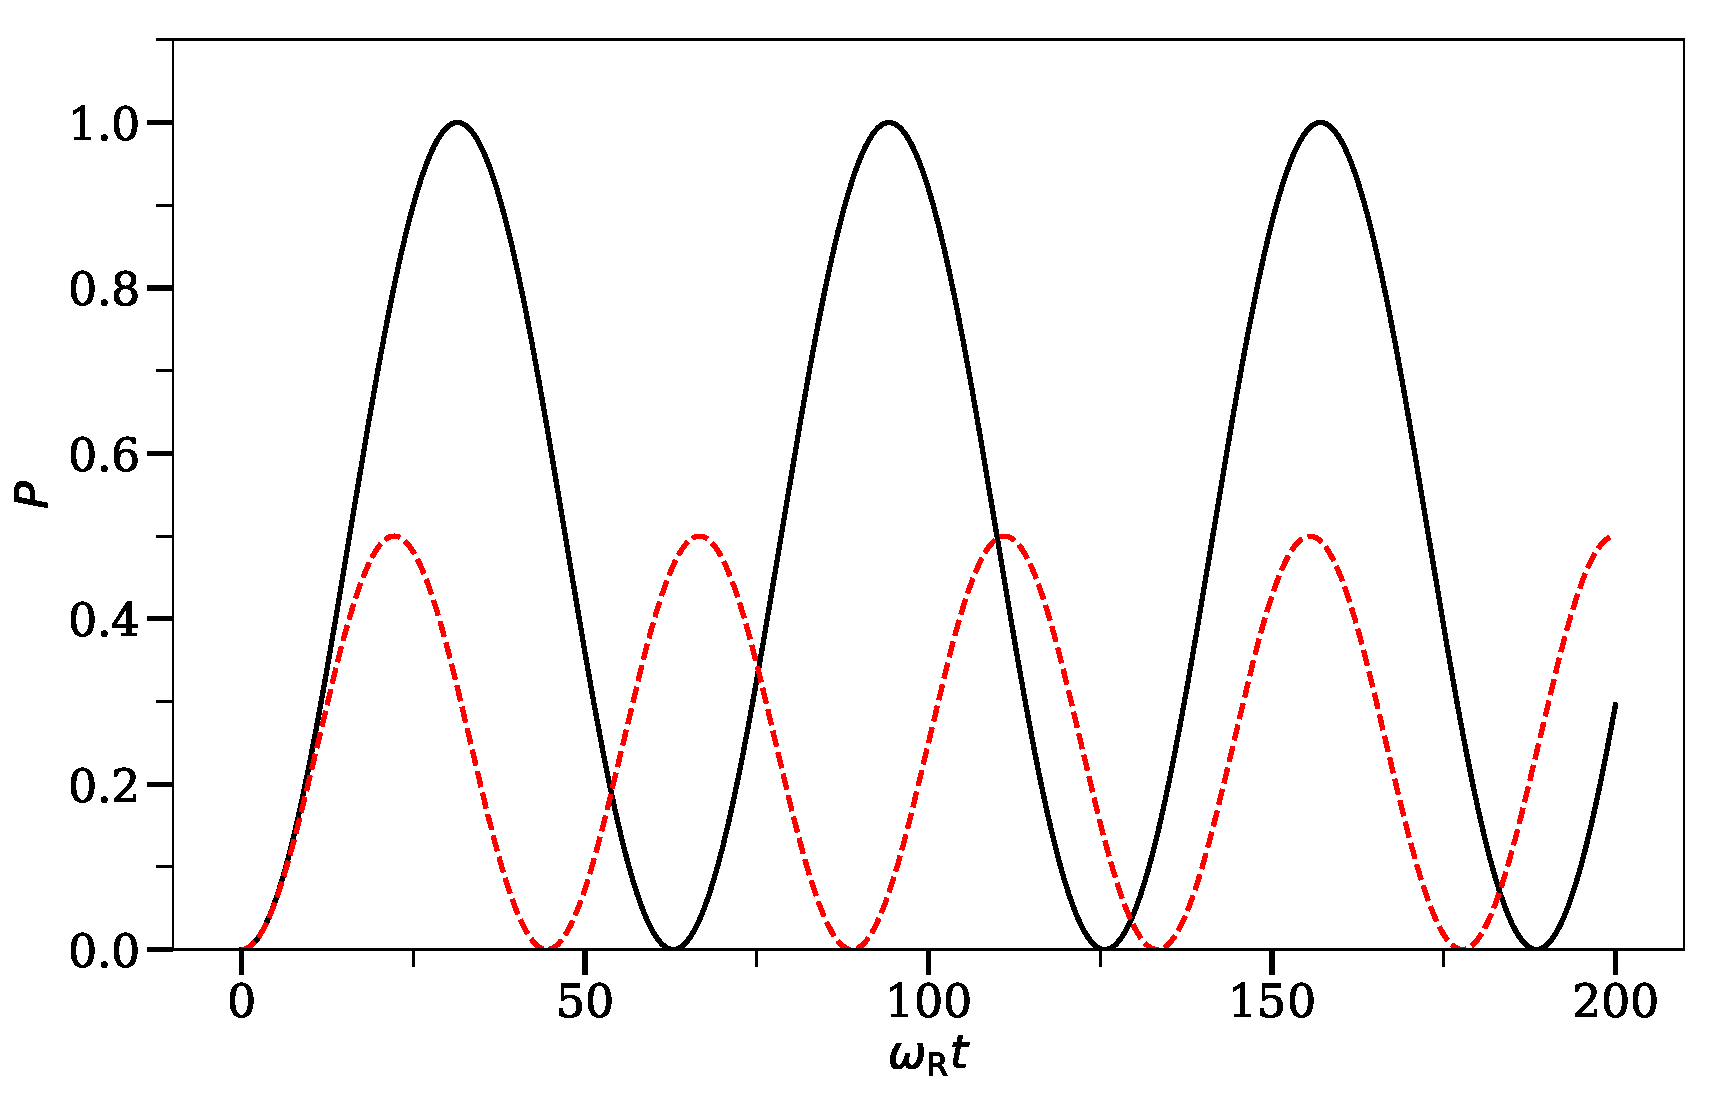
\includegraphics[width=\textwidth]{chapters/assets/app/rabi-oscillations}
    \caption{Rabi oscillations for two different incoming light frequencies. $k_\RR/\omega_\RR=1$ is the resonance condition. For $k_\RR/\omega_\RR=1.1$,  the oscillation amplitude is 0.5. I have used $A_\RR=0.1$ in both calculations. }
    \label{app-fig:rabi-examples}
\end{figure}

Similar to neutrino oscillations in a uniform matter profile (see Eqn.~\ref{chap:basics-sec:flavor-isospin-pic-fig:msw-adiabatic-critical}), resonance of Rabi oscillations occurs when the term $\vec{H}_3$ disappears in this corotating frame. The state vector $\vec{s}$ converts from $+1/2$ (low energy state) to $-1/2$ (high energy state) completely. The detuning, which is defined by $k_{\mathrm{R}} - \omega_{\mathrm R}$, determines how off-resonance the system is. The amplitude of driving field $A_{\mathrm{R}}$ determines the resonance width,
\begin{align}
\text{Detuning} =&~\lvert k_{\mathrm{R}} - \omega_{\mathrm R} \rvert, \\
\text{Resonance Width} =&~\lvert A_{\mathrm R} \rvert.
\end{align}
The width of the resonance is also explained in Fig.~\ref{app-fig:rabi-resonance-width}. We also notice that the transition amplitude is determined by relative detuning $\RD$, which is defined as
\begin{equation}
    \RD = \left\lvert \frac{ k_{\mathrm R} - \omega_{\mathrm R}}{A_{\mathrm R}} \right\rvert.
    \label{chap:app-sec:rabi-oscillations-eqn:relative-detuning-def}
\end{equation}

\begin{figure}[htbp]
    \centering
    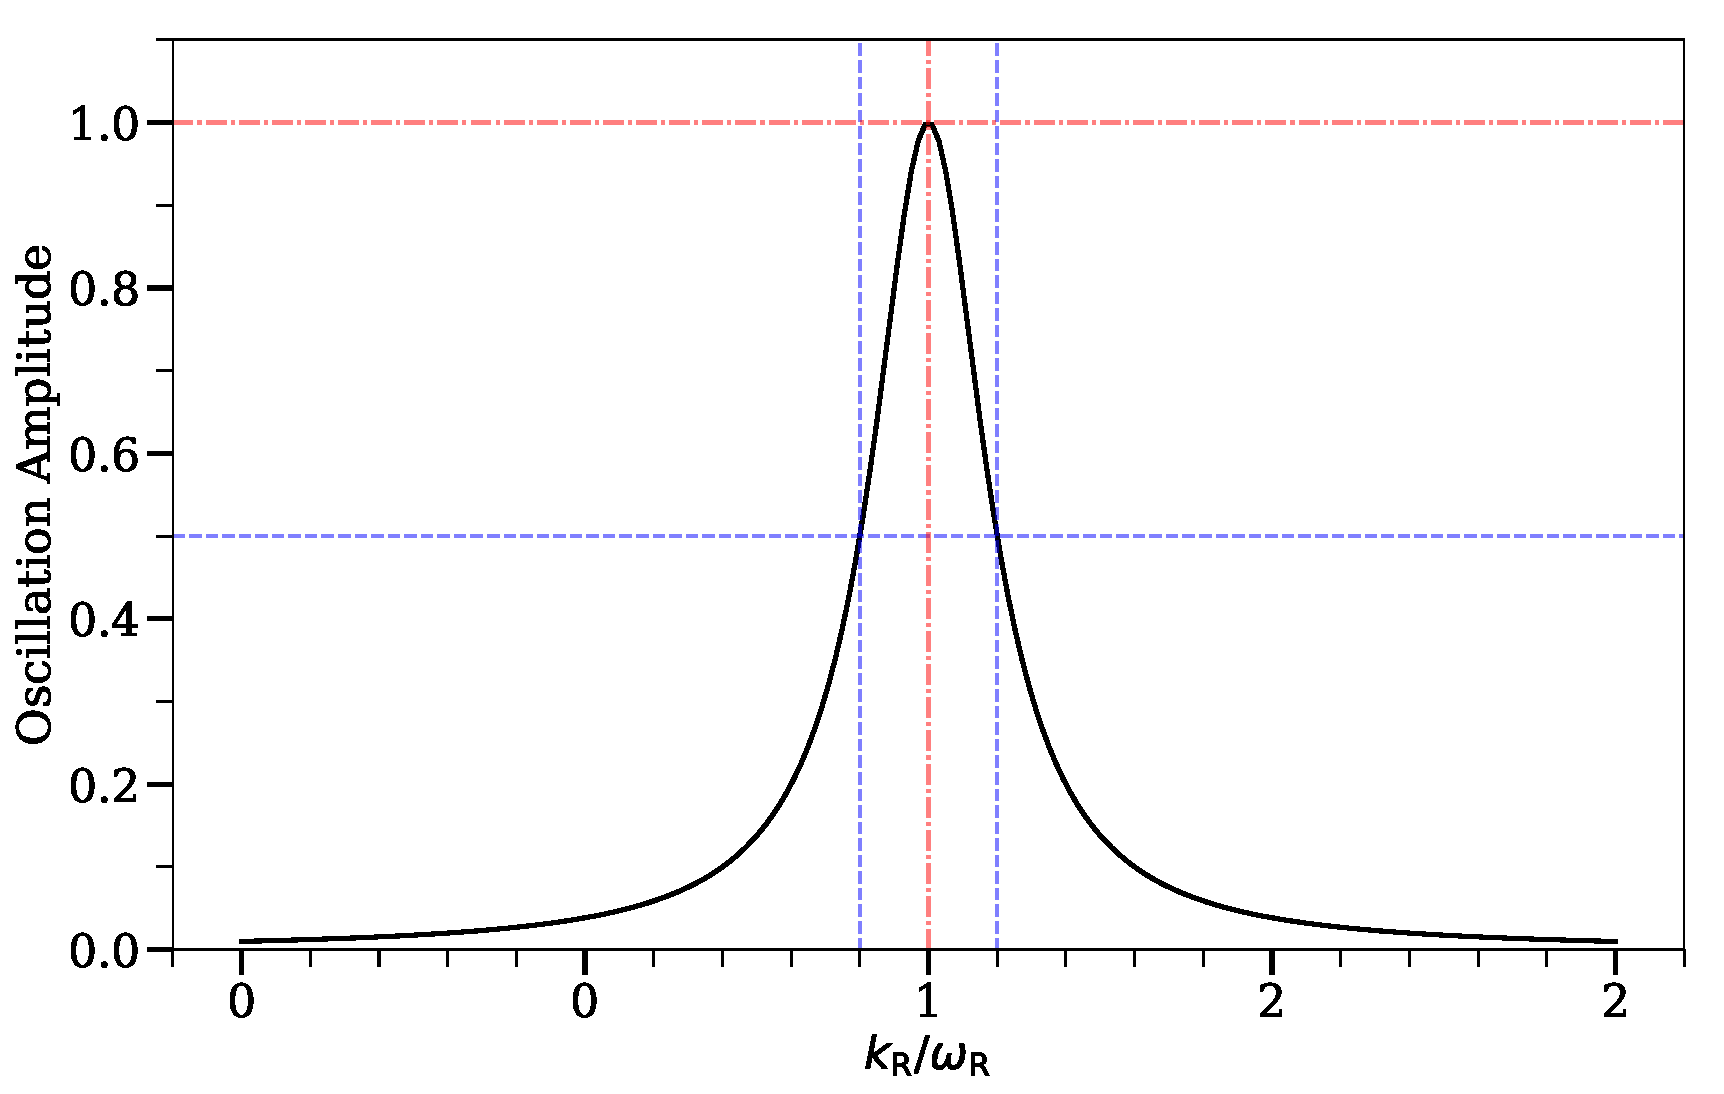
\includegraphics[width=\textwidth]{chapters/assets/app/rabi-resonance-width}
    \caption{Rabi oscillations for different driving frequencies $k_\RR$ in unit of $\omega_\RR$. The maximum amplitude occurs at $k_\RR/\omega_0=1$. Resonance width is defined to be the width where amplitude becomes half of the maximum which is sandwiched by blue-dashed vertical grid lines. The red-dash-dotted vertical grid line indicates the maximum amplitude.}
    \label{app-fig:rabi-resonance-width}
\end{figure}


In many problems, the two-level quantum system has more than one driving frequencies. Here I will explain the Rabi formula that we derived for Rabi oscillation problem with two driving potentials, which has a Hamiltonian of the form
\begin{align*}
    \mathsf H_{\mathrm R} =& -\frac{\omega_{\mathrm R}}{2}\sigma_3 - \frac{A_{1} }{2}  \left( \cos(k_{1} t +\phi_{1})\sigma_1  - \sin(k_{1} t +\phi_{1}) \sigma_2\right) \nonumber\\
    & - \frac{A_{2} }{2}  \left( \cos(k_{2} t +\phi_{2})\sigma_1  - \sin(k_{2} t +\phi_{2}) \sigma_2\right).
\end{align*}
I decompose it into $\vec{H}_{\mathrm R}=\vec{H}_3 + \vec{H}_{1} + \vec{H}_2$, where
\begin{equation*}
    \vec{H}_1 =  \begin{pmatrix}
     A_{1} \cos(k_{1}t+\phi_{1}) \\
     -A_{1} \sin(k_{1}t+\phi_{1})  \\
     0
   \end{pmatrix},   \vec{H}_2 =  \begin{pmatrix}
     A_{2} \cos(k_{2}t+\phi_{2}) \\
     -A_{2} \sin(k_{2}t+\phi_{2})  \\
     0
      \end{pmatrix}.
\end{equation*}
Assume $\vec{H}_1$ is the on-resonance perturbation which means that $k_1 = \omega_{\mathrm{R}}$. The three terms are defined as $\vec H_3$, $\vec H_1$, and $\vec H_2$ respectively. $\vec H_1$ and $\vec H_2$ are two rotating vectors as a function of $r$ with frequencies $k_1$ and $k_2$ in this vector space, while $\vec H_3$ is perpendicular to $\vec H_1$ and $\vec H_2$.

The most general condition that we can drop the new perturbation $\vec{H}_2$ is to make sure $k_2$ is far from the resonance condition compared to the resonance width,
\begin{equation}
\RD \equiv \frac{\lvert k_2 -\omega_{\mathrm R}\rvert}{\lvert A_2\rvert} \gg 1.
\end{equation}
In fact, I will derive a more stringent criteria to neglect the second driving potential using the idea of energy gap shift.
% The transition amplitude between the two states becomes
% \begin{equation}
% P(t) = \frac{1}{1+\RD^2}\sin^2\left(\frac{\Omega_{\mathrm{R}}}{2}t\right).
% \end{equation}
% \begin{figure}[htbp]
%     \centering
%     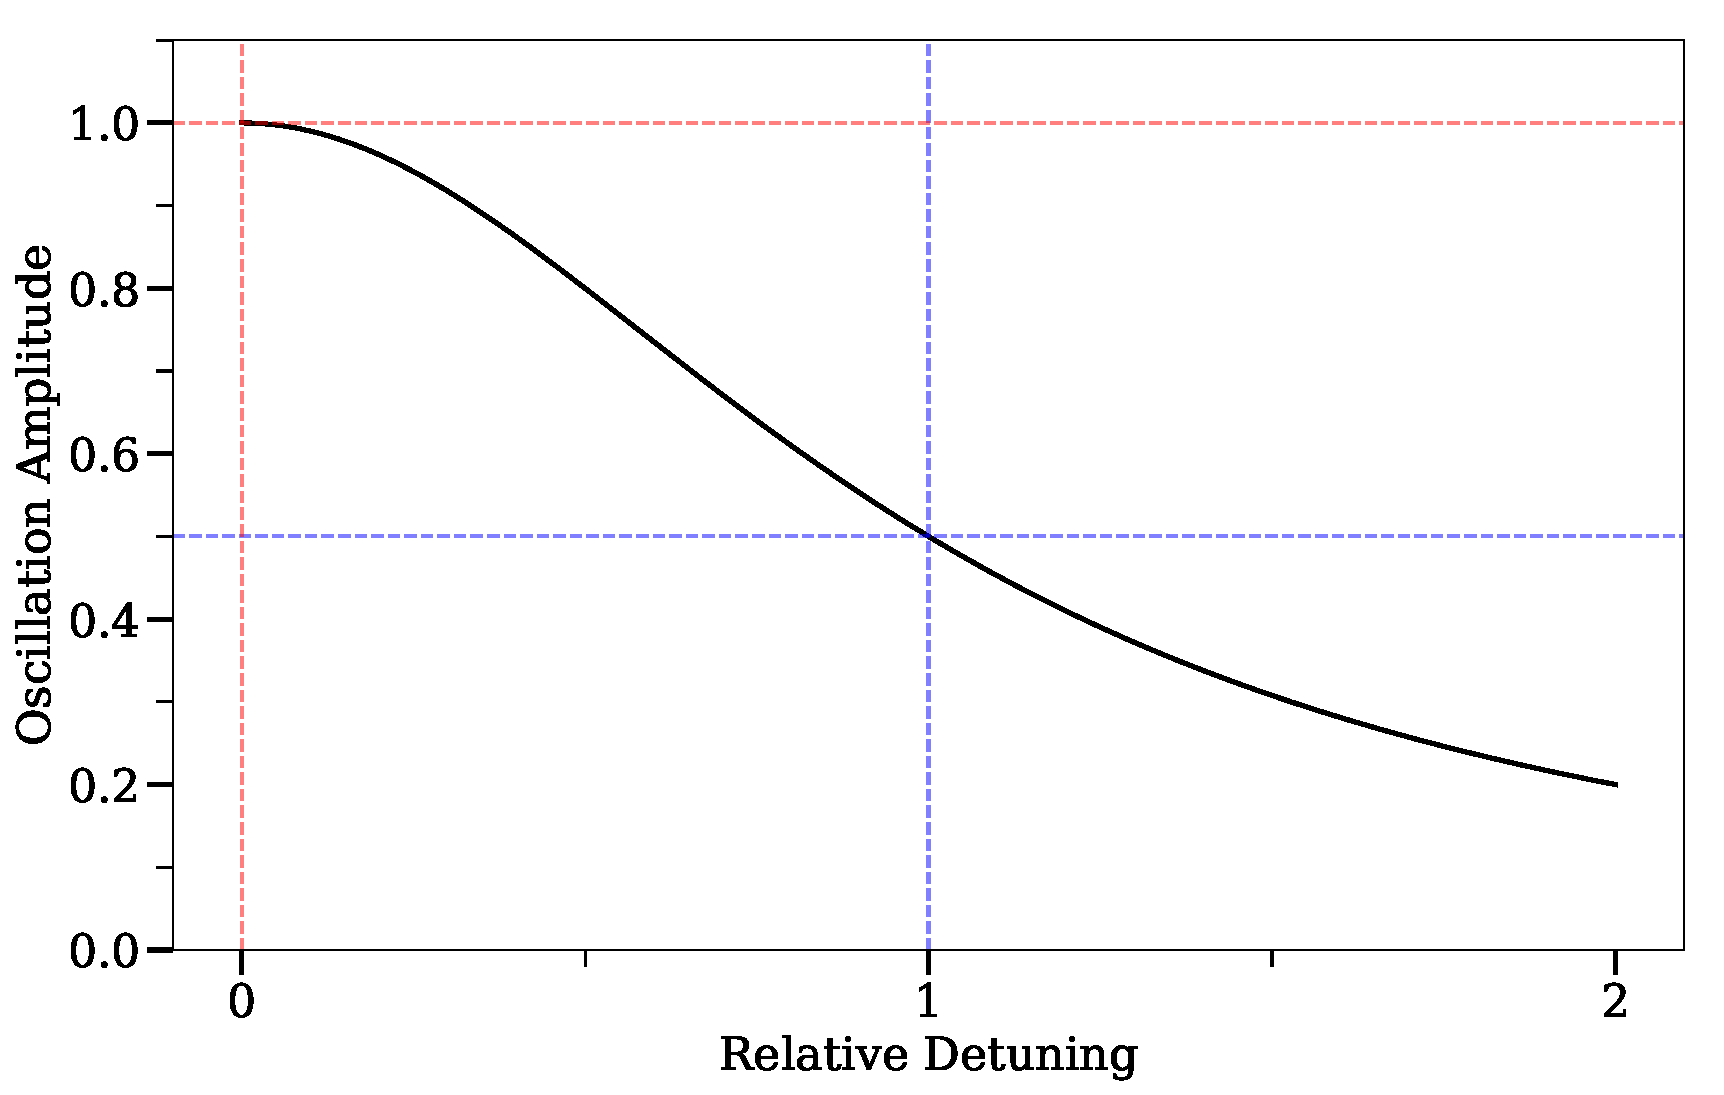
\includegraphics[width=\textwidth]{chapters/assets/app/rabi-resonance-detuning}
%     \caption{Rabi oscillations for two different relative detunings $\RD$. $\RD=1$ is the resonance condition. The amplitude reach maximum when $\RD=0$, i.e., $k_\RR=\omega_\RR$. }
%     \label{app-fig:rabi-resonance-width}
% \end{figure}
%Suppose I have a Rabi oscillation system with two modes, one of which is at resonance with frequency $k_1=\omega_{\mathrm m}$ and the other mode with frequency $k_2$ that is off resonance. In some cases, there can be a significant transition amplitude decrease because of the off resonance frequency $k_2$, which can be interpreted as shift of energy gap due to the frequency $k_2$.
% To model the effect, I construct a Rabi oscillation Hamiltonian with two modes of different frequency,
% \begin{equation}
% \mathsf H^{(\mathrm{m})}  = -\frac{\omega_{\mathrm{m}}}{2} \sigma_3 - \frac{1}{2} \sum_{n=1}^N  A_n \cos (k_n r) \sigma_1 + \frac{1}{2} \sum_{n=1}^N  A_n \sin (k_n r) \sigma_2,
% \label{eq-hamiltonian-rabi-two-modes-interference}
% \end{equation}
% where $N=2$ for two frequency case. To show the destruction effect, the Hamiltonian Eqn.~\ref{eq-hamiltonian-rabi-two-modes-interference} is reformulated into a vector in flavor-isospin space,
% \begin{equation}
% \mathbf H = \mathbf H_3 + \mathbf H_1 +\mathbf H_2 = \begin{pmatrix}
% 0\\
% 0\\
% \omega_\mm
% \end{pmatrix} + \begin{pmatrix}
% A_1 \cos (k_1 r)\\
% -A_1 \sin (k_1 r)\\
% 0
% \end{pmatrix} + \begin{pmatrix}
% A_2 \cos (k_2 r)\\
% -A_2 \sin (k_2 r)\\
% 0
% \end{pmatrix}.
% \end{equation}
To work out the energy gap shift, we go to the frame that corotates with $\vec H_2$, in which we have the new frequencies $k_1'=k_1-k_2$ and $k_2'=0$ as well as new energy gap $\omega_{\RR}' = \omega_{\RR}- k_2$. The resonance mode $\vec H_1$ retains on the resonance condition since $k_1'=\omega_{\RR}'$, i.e. $k_1-k_2 = \omega_{\RR}-k_2$, holds in the new frame. On the other hand, we have two static fields $\vec H_3$ and $\vec H_2$ together as the new energy gap, as long as $\vec H_2\ll \vec H_3$, which is the usual case. The new energy gap in this frame is calculated as
\begin{align}
    \tilde\omega_{\mathrm{R}}' =& \sign (\omega_{\mathrm R}') \sqrt{\omega_{\mathrm{R}}'^2 + A_2^2 } \nonumber\\
    \approx & \omega_{\mathrm{R}}' + \frac{A_2^2}{2\omega_{\mathrm R}'} \nonumber\\
    =& \omega_{\mathrm R} - k_2 + \frac{1}{2}\frac{A_2^2}{\omega_{\mathrm R} - k_2},
    \label{eq-new-energy-gap-due-to-second-mode-approximation}
\end{align}
where we kept only first order of Taylor series. The Taylor expansion in Eqn.~\ref{eq-new-energy-gap-due-to-second-mode-approximation} holds as long as the relative detuning for the second frequency is large which means the second frequency is off resonance. As an approximation, the transitions between the two energy states follows the Rabi oscillations with energy gap $\tilde \omega_{\mathrm R}'$ and driving field with frequency $k_1'=k_1-k_2$. Consequently, we can estimate how much the amplitude of the transition is suppressed due to $k_1$ mode by calculating the new relative detuning,
\begin{align}
    \RD' =& \frac{\lvert k_1' - \tilde \omega_{\mathrm R}' \rvert}{\lvert A_1 \rvert}\nonumber\\
    =& \left \lvert \frac{ k_1-\omega_{\mathrm R}}{ A_1} + \frac{ A_2^2 }{2  A_1 ( k_2 - \omega_{\mathrm R})} \right  \rvert\\
    =& \left \lvert  \frac{\sign({ k_1-\omega_{\mathrm R}})}{\sign (k_2 - \omega_{\mathrm R})} \RD_1 +  \frac{ A_2 }{2 A_1 \RD_2 }\right \rvert ,
    \label{app:chap:matter-eq:relative-detuning-changed}
\end{align}
where $\RD_1$ and $\RD_2$ are the relative detuning of the first mode and second mode, respectively. They are defined as
\begin{equation*}
\RD_i =  \left\lvert \frac{ k_i - \omega_{\mathrm R}}{A_i} \right \rvert.
\end{equation*}
In principle, the energy gap of the first frequency can be changed to approach the resonance or escape the resonance by carefully arranging the second frequency, which is also obvious from Eqn.~(\ref{chap:matter-eq:relative-detuning-changed}). For the purpose of the section we first discuss the most important destruction effect by choosing $\RD_1 = 0$. We observe the importance of the relative detuning. For the second mode to significantly interfere with the first mode, we need a small $\RD_2$ and a large amplitude or width $A_2\gg A_1$.


%%%%%%%%%%%%%%%%%%%%%%%%%%%%%%%%%%%%
%%%%%%%%% Rabi oscillation
%%%%%%%%%%%%%%%%%%%%%%%%%%%%%%%%%%%%
\subsection{\label{chap:matter-sec:single-frequency-matter-profile}Single Frequency Matter Profile}


I will examine the neutrino flavor conversions in a single frequency matter profile $\delta\lambda(r) = \lambda_1 \cos(k_1 r)$. The Hamiltonian in background matter basis becomes
\begin{equation}
\mathsf H^{(\mm)} = - \frac{\omega_\mm}{2}\sigma_3  + \frac{1}{2} \lambda_1 \cos(k_1 r) \cos 2\theta_\mm \sigma_3 - \frac{1}{2} \lambda_1 \cos(k_1 r)\sin 2\theta_\mm \sigma_1.
\label{eq-hamiltonian-bg-matter-basis-single-frequency}
\end{equation}
As will be proved later, the varying $\sigma_3$ term $\frac{1}{2} \lambda_1 \cos(k_1 r) \cos 2\theta_\mm \sigma_3$ in the above Hamiltonian, which is the varying energy gap due to varying matter density fluctuations, has little effect on the transition probabilities when the system is not too far from resonance\footnote{For the purpose of this section, I will consider the case when $k_1$ is not far away from resonance.}. With the varying $\sigma_3$ term removed, the single frequency matter perturbation neutrino flavor conversion system will be reduced to a Rabi oscillation system. The external driving field frequency is $\pm k_1$ and the energy gap is $\omega_{\mathrm m}$. I can decompose $\cos( k_1 r )$ into two exponential functions so that we have two external driving frequencies $k_1$ and $-k_1$. By neglecting the off-resonance frequency $-k_1$, the Hamiltonian can be simplified to
\begin{align}
\mathsf H^{(\mathrm{m})} \to & -\frac{\omega_{\mathrm m}}{2} \sigma_3  - \frac{1}{2} \lambda_1 \sin 2\theta_{\mathrm m} \cos( k_1 r ) \sigma_1\label{eq-hamiltonian-bg-matter-basis-single-frequency} \\
\to & -\frac{\omega_{\mathrm m}}{2} \sigma_3  - \frac{1}{2} A_1 \exp (\mathrm ik_1 r) \sigma_1 \nonumber \\
= & -\frac{\omega_{\mathrm m}}{2} \sigma_3  - \frac{1}{2} A_1 \cos ( k_1 r)  \sigma_1 + \frac{1}{2} A_1\sin(k_1 r) \sigma_2,\nonumber
\label{chap:matter-sec:single-frequency-matter-profile-eqn:single-frequency-hamiltonian-approximation}
\end{align}
where I have used
\begin{equation}
A_1 = \frac{\lambda_1 \sin 2\theta_{\mathrm m} }{2}.
\label{eq-define-a1}
\end{equation}



Now I have reduced the neutrino oscillations to Rabi oscillations. The resonance happens when the energy gap $\omega_{\mathrm m}$ is close to the external driving field frequency $k_1$, i.e., $\omega_{\mathrm m} \sim k_1$. As long as the resonance condition is satisfied, the transition probability between the two mass states should be predicted well using Rabi formula.
To show that this conjecture of simplifying neutrino flavor conversions to Rabi oscillations is correct, I calculated the transition probabilities of the neutrinos described by Eqn.~\ref{eq-hamiltonian-bg-matter-basis-single-frequency} numerically, and compared them with Rabi formula Eqn.~\ref{app:rabi-system-transition-probability} from the Rabi oscillations described by Eqn.~\ref{rabi-oscillation-single-perturbation}.

\begin{figure}[h!tbp]
                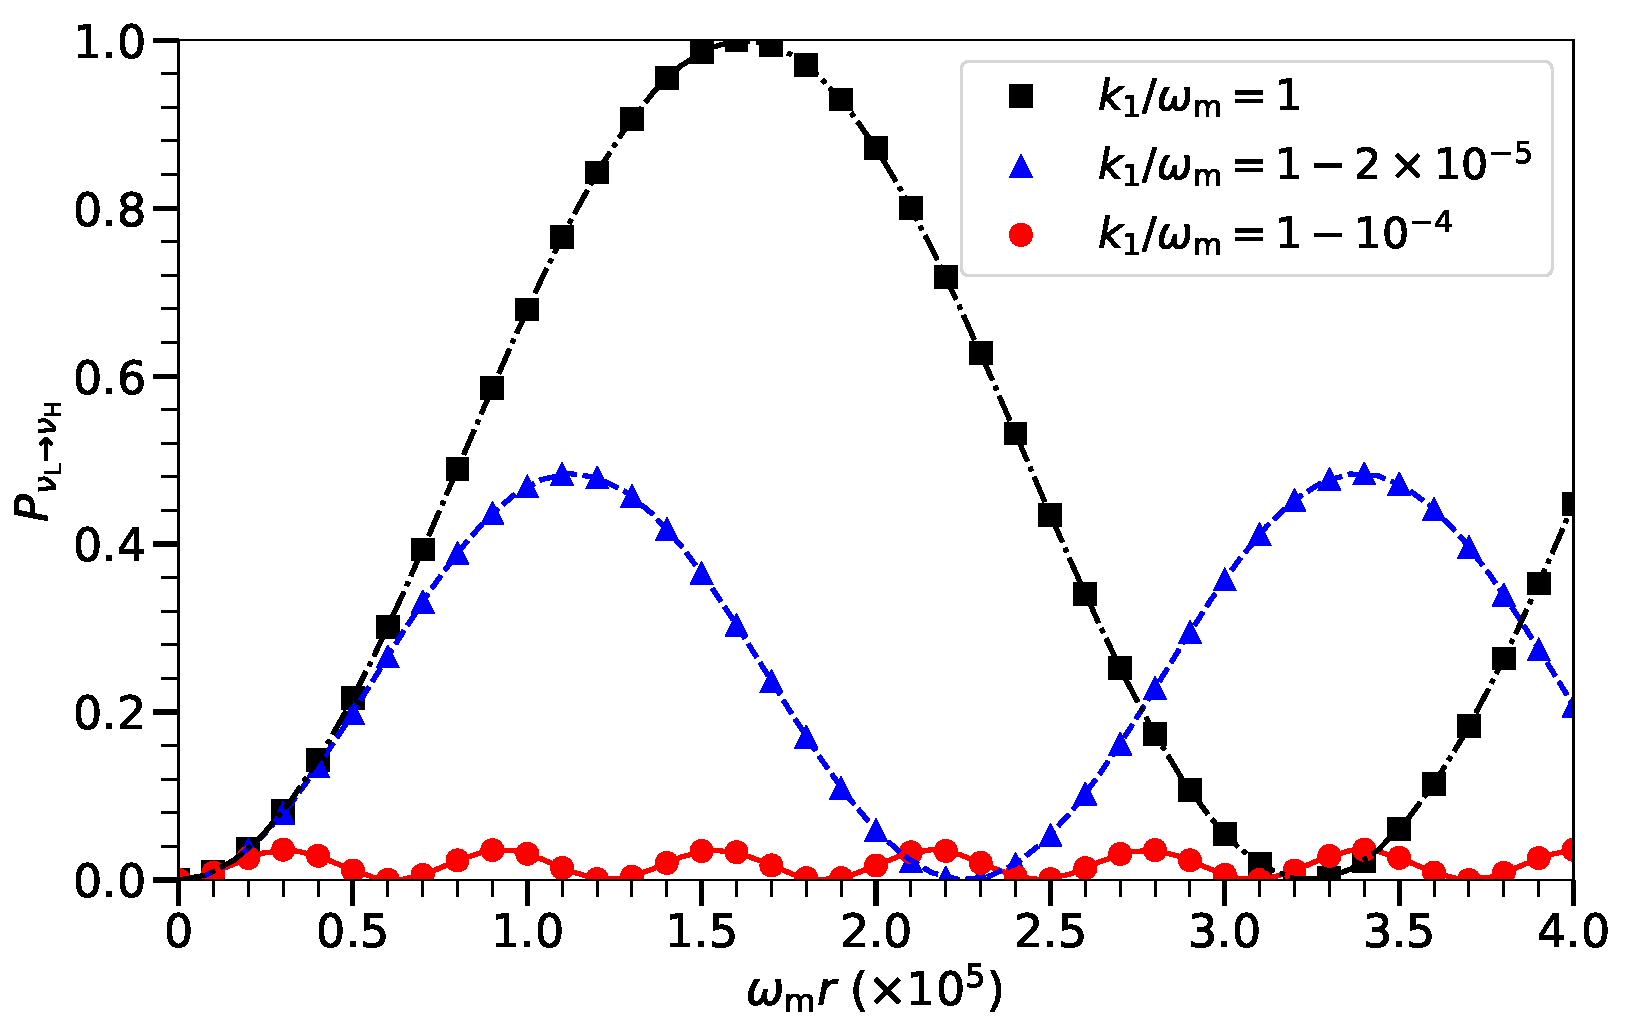
\includegraphics[width=\columnwidth]{chapters/assets/rabi/rabiOscillationsNeutrinoCoincidence-single-frequency}
                %rabiOscillationsNeutrinoCoincidence}
                \caption{Single frequency matter profile and Rabi oscillation. The markers are numerical results for the transition probabilities between two background mass eigenstates for the neutrinos with matter perturbation $A_1\sin(k_1 r)$. The dots, diamonds, and squares are for $k_1=\omega_{\mathrm m}$, $k_1=(1-2\times 10^{-5})\omega_{\mathrm m}$, and $k_1=(1-10^{-4})\omega_{\mathrm m}$ respectively. The lines are the predictions using Rabi formula. During the calculation, $\lambda_0$ is set to $0.5$ of the MSW resonance potential $\lambda_{\mathrm{MSW}}=\omega_{\mathrm{v}}\cos 2\theta_{\mathrm v}$ and mixing angle is chosen so that $\sin^2(2\theta_{\mathrm v}) = 0.093$.}
                \label{fig-rabiOscillationsNeutrinoCoincidence}
\end{figure}

In Fig.~\ref{fig-rabiOscillationsNeutrinoCoincidence}, I have plotted the numerical results using markers as well as the prediction using Rabi formula using lines. The agreement between numerical solutions of neutrino transitions between mass states and Rabi formula will be explained more precisely in Sec.~\ref{sec:jacobi}. For now, we address the significance of relative detuning $\RD = \lvert k_1 - \omega_{\mathrm m} \rvert /\lvert A_1 \rvert$,  which is rigoriously defined in Eqn.~\ref{chap:app-sec:rabi-oscillations-eqn:relative-detuning-def}. $\RD\to 0$ indicates that the neutrino oscillation is very close to resonance, while $\RD\to \infty$ indicates that the neutrino oscillation is far away from resonance. The corresponding relative detunings in Fig.~\ref{fig-rabiOscillationsNeutrinoCoincidence} are $0$, $1.0$, and $5.2$ for $k_1=\omega_{\mathrm{m}}$, $k_1=(1-2\times 10^{-5})\omega_{\mathrm m}$, and $k_1=(1-10^{-4})\omega_{\mathrm m}$.

% 0, 0.516197,1.03239,5.16197

For a single-frequency perturbation in the matter profile $\lambda(r) =\lambda_1 +  \lambda_1\sin(k_1 r)$, P. Krastev and A. Smirnov concluded that the parametric resonance condition is $\omega_{\mathrm{m}} \sim n k_1$, if instantaneous $\omega_{\mathrm{m,inst}}(r)$ associated with the matter profile at distance $r$ varies slowly~\cite{Krastev1989}. This condition is exactly the Rabi resonance condition when $n=1$, as such condition matches the driving field frequency to the energy split. Higher order effects are explained in Sec.~\ref{sec:single-revisted}.





\section{\label{chap:matter-sec:multiple-matter-frequencies}Multi-frequency Matter Profiles}


The approach applied to single frequency matter profile also helps with the understanding of multi-frequency matter profile. However, multi-frequency matter profile leads to multiple modes of Rabi oscillations, even with our simplified approach by dropping the varying $\sigma_3$ term in Hamiltonian. In this section, we examine the neutrino oscillations in multi-frequency matter profiles using the interference effects discussed in Sec.~\ref{chap:app-sec:rabi-oscillations}.
%Castle wall matter profile will serve as an example of multi-frequency profile to illustrate the idea of interference.



%%%%%%%%%
%%%% Interference
%%%%%%%%



%\subsection{\label{sec:interference-with-long-wavelength-mode}Interference Between Different Frequencies}

% \fbox{
% \parbox{0.9\columnwidth}{
% \begin{itemize}
%     \item Two limits: strong interference regime and low-interference regime
%     \item For strong interference we include multiple modes
%     \item For weak interference, we can interpret the case that one of the matter profile wavelength is much larger than the other. In this case we have a shift of background matter density of the short wavelength perturbation profile.
%     \item Examples. A slight shift in the background density could remove the resonance, which can be quantified.
%     \begin{equation*}
%         a
%     \end{equation*}
% \end{itemize}
% }
% }

The Hamiltonian for neutrino oscillations in matter background with two frequencies is
\begin{align}
  \mathsf H^{(\mm)} =& - \frac{\omega_\mm}{2}\sigma_3  + \frac{1}{2} \left( \lambda_1 \cos(k_1 r) + \lambda_2 \cos(k_2 r) \right) \cos 2\theta_\mm \sigma_3 \nonumber\\
   &- \frac{1}{2} \left( \lambda_1 \cos(k_1 r) + \lambda_2 \cos(k_2 r)\right)\sin 2\theta_\mm \sigma_1.
  \label{eq-hamiltonian-bg-matter-basis-multi-frequency}
\end{align}
I will drop the varying $\sigma_3$ terms for the same reason as in single frequency matter profile case. The Hamiltonian becomes the two-frequency Rabi oscillation Hamiltonian,
\begin{equation}
  \mathsf H^{(\mm)} = - \frac{\omega_\mm}{2}\sigma_3  - \frac{1}{2} \left( \lambda_1 \cos(k_1 r) + \lambda_2 \cos(k_2 r)\right)\sin 2\theta_\mm \sigma_1.
  \label{eq-hamiltonian-bg-matter-basis-multi-frequency-drop-varying-sigma3}
\end{equation}
The oscillation probabilities can be predicted by the Rabi formula Eqn.~\ref{app:rabi-system-transition-probability} with the new relative detuning calculated with Eqn.~\ref{app:chap:matter-eq:relative-detuning-changed}. It can be verified by comparing the numerical solution and estimation using Rabi formula. However, I am most interested in the amplitude change due to $\mathbf H_2$ mode. Relative detuning is the only variable that I need to calculate the amplitude, hence I only compare the numerical results with estimated amplitudes using $1/(1+\RD'^2)$.
To verify the condition, I choose the first rotating perturbation to satisfy the resonance condition $k_1=\omega_{\mathrm{m}}$, the condition for the second rotating field shifting the system out of resonance is that the relative detuning becomes larger than $1$, which leads to
\begin{equation}
\lvert A_2 \rvert \geq \sqrt{2\omega_{\mathrm{m}} \lvert A_1 (k_2-\omega_{\mathrm m})\rvert} \equiv A_{2,\mathrm{Critical}}.
\end{equation}
I expect the transition amplitude to decrease as we have larger $\lvert A_2\rvert$.


\begin{figure}[!htbp]
                \centering
                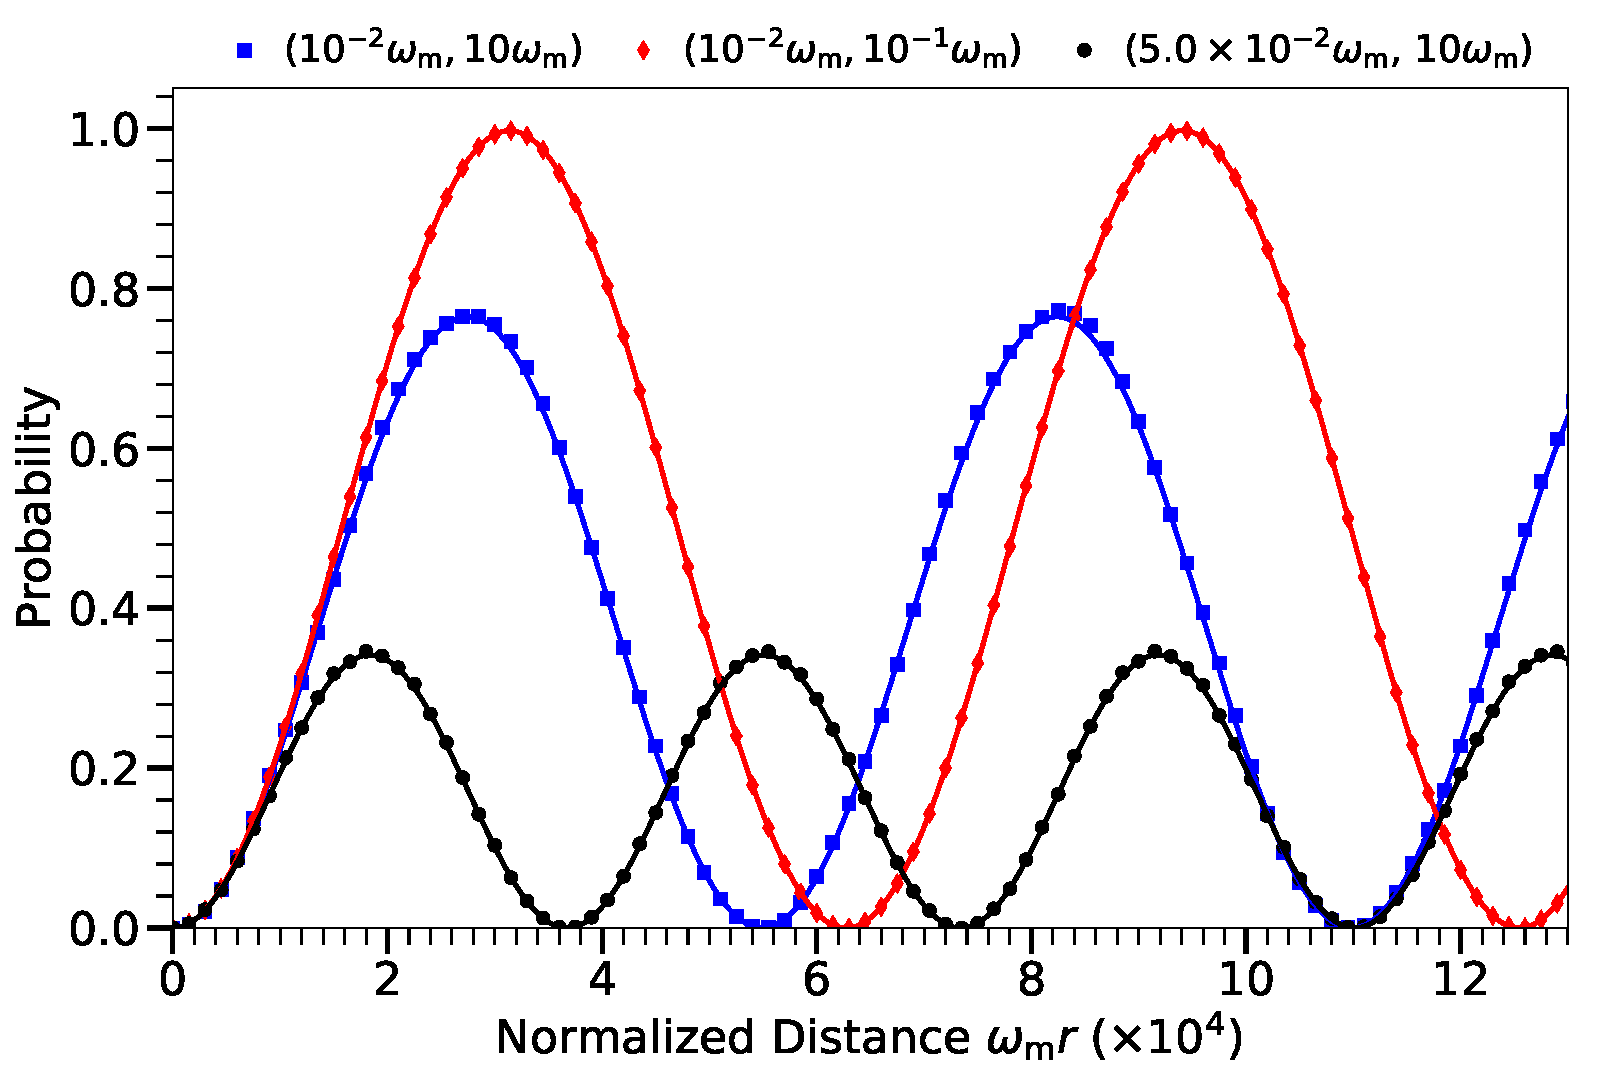
\includegraphics[width=\columnwidth]{chapters/assets/matter/interference-reduction-slide-with-legend}
                \caption{Reduction of transition amplitudes due to interference. Blue squares, red diamonds, and black dots are for $A_2=10^{-2}\omega_{\mathrm{m}}$, $k_2=10\omega_{\mathrm m}$, $A_2=10^{-2}\omega_{\mathrm{m}}$, $k_2=10^{-1}\omega_{\mathrm m}$, $A_2=5.0\times, and 10^{-2}\omega_{\mathrm{m}}$, $k_2=10\omega_{\mathrm m}$, respectively. The lines are the corresponding Rabi formula predictions. In all the calculations, I used $A_1=10^{-4}\omega_{\mathrm m}$, $k_1=\omega_{\mathrm m}$. During the calculations, $\Lambda_0$ is set to half of the MSW resonance potential, $\Lambda_0 = \frac{1}{2}\lambda_{\mathrm{MSW}}=\frac{1}{2}\omega_{\mathrm{v}}\cos 2\theta_{\mathrm v}$.}
                \label{fig-rabi-oscillations-energy-gap-change}
\end{figure}


I choose the two modes where the first one has amplitude $A_1 = 10^{-4}\omega_{\mathrm{m}}$ and frequency $k_1 = \omega_{\mathrm{m}}$. With a small amplitude of the second frequency, $A_2=10^{-4}\omega_{\mathrm{m}}$, and large frequency $k_2=10\omega_{\mathrm{m}}$, I obtain almost full resonance. As shown in Eqn.~\ref{app:chap:matter-eq:relative-detuning-changed}, larger $A_2$ leads to more effective destruction effect. In Fig.~\ref{fig-rabi-oscillations-energy-gap-change}, I am showing the full numerical solution of neutrino oscillations in two-frequency matter background, and the prediction of oscillations using Rabi formula, which is a good match to the numerical results. To show the importance of relative detuning, I also calculated the relative detuning for each cases, which are $0.06$, $0.6$, $1.4$ for the lines from top to down. Notice that the width of each cases doesn't change since I kept $A_1$ fixed for each calculation, which indicates that the decreasing in transition amplitude is because of the increasing in detuning.

% \subsection{\label{chap:matter-sec:constructive}Constructive Effects}
\begin{figure}[!htbp]
    \centering
    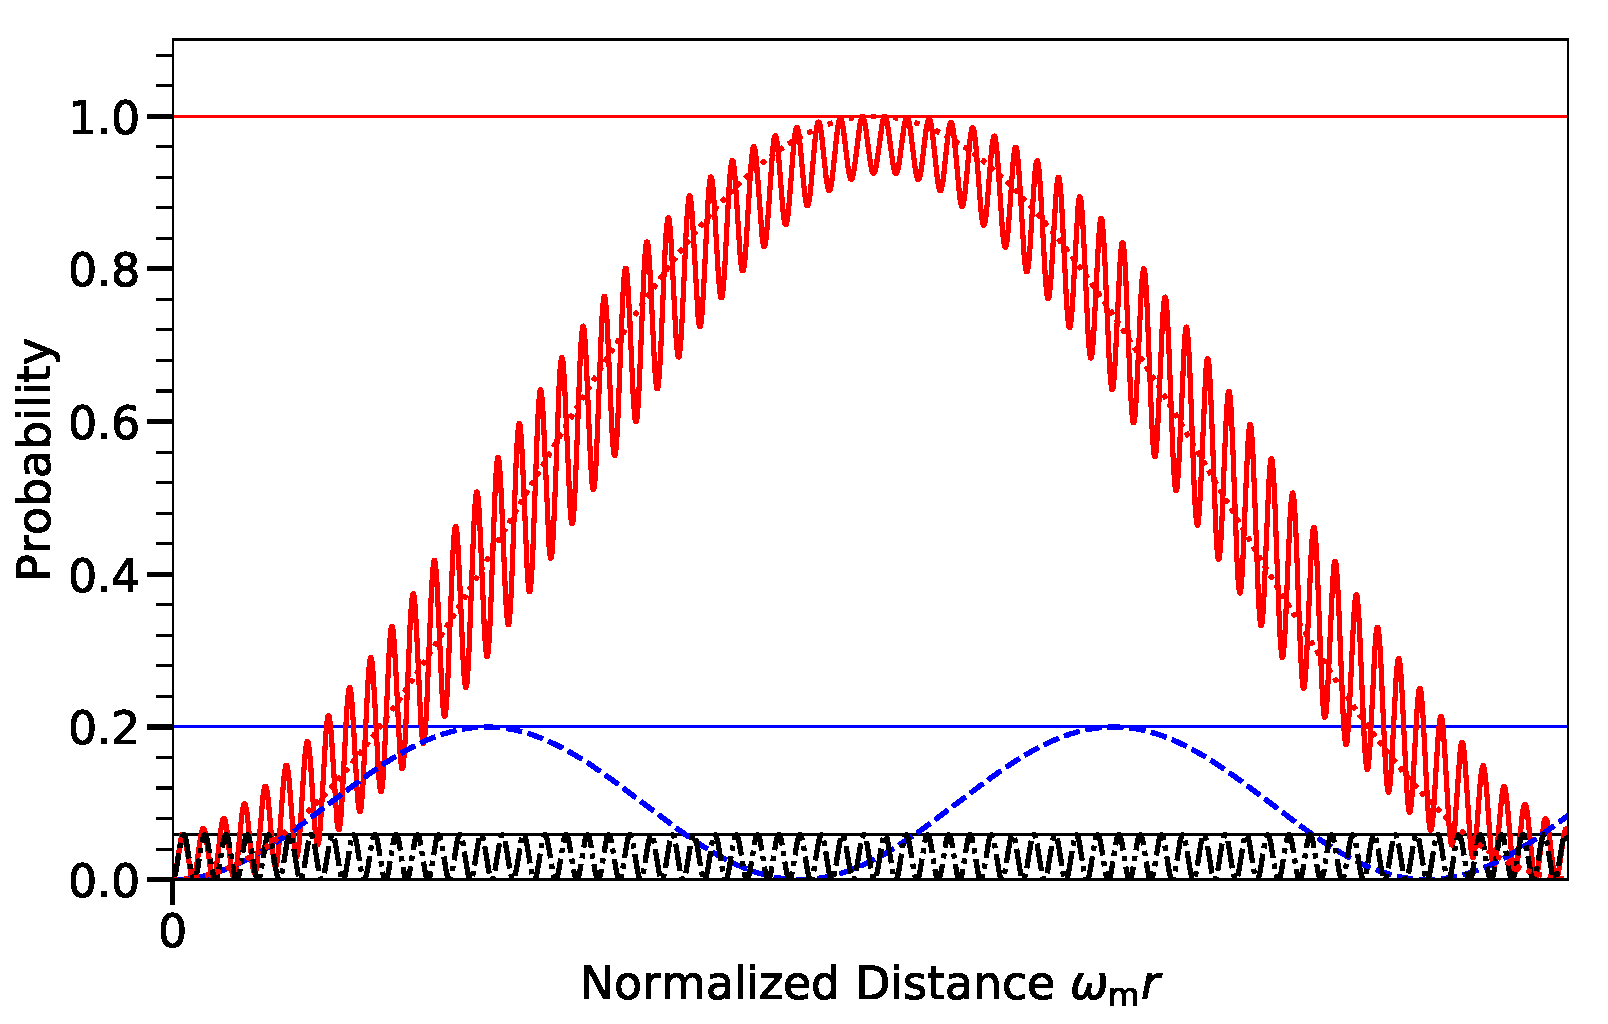
\includegraphics[width=\textwidth]{chapters/assets/rabi/rabiOscillationsNeutrinoCoincidence-two-frequencies-constructive.pdf}
    \caption{Constructive interference for two frequencies in matter density profile. The solid red line, dashed blue line, dash-dotted black line, are the transition probability for two frequencies combined, the first frequency $k_1$ only, the second frequency $k_2$ only. The amplitudes of each frequency are $A_1=0.4$, $A_2=2.6$ respectively. The grid lines are the oscillations amplitudes predicted by Rabi formula. The dotted red line is the oscillations predicted by Rabi formula for the two combined frequencies.}
    \label{chap:matter-sec:constructive-fig:two-frequencies-constructive}
\end{figure}

Adding a second frequency to the matter density profile can also be constructive. I calculated an example with two frequencies in matter density profile, so that the Hamiltonian is
\begin{equation*}
    \mathsf H^{(\mm)} = - \frac{\omega_{\mathrm m}}{2} \sigma_3 - \left(\frac{A_1}{2}\cos(k_1 r) + \frac{A_2}{2}\cos(k_2 r) \right) \sigma_1 + \left( \frac{A_1}{2}\sin(k_1 r) + \frac{A_2}{2}\sin(k_2 r) \right) \sigma_2.
\end{equation*}
I choose two matter profile frequencies that are off resonance and producing large relative detuning,
% k1_0.95_k2_2.6_a1_0.025_a2_0.4
\begin{equation}
    A_1 = 0.025, \qquad k_1 = 0.95, \qquad A_1 = 0.4, \qquad k_2 = 2.6.
\end{equation}
The oscillation amplitude for each mode being much smaller than 1. However, the combined two frequencies case produces oscillations are resonance (c.f.~Fig.~\ref{chap:matter-sec:constructive-fig:two-frequencies-constructive}), since the relative detuning for the combined two frequencies case is 0.



%%%%%%%%%%%%%%%%%%%%%%%%%%%%%%%%%%%%%%%%%%%%%%%%%%%%
%%%%%%%%%  Jacobi Anger Expansion  %%%%%%%%%%%%%%%%%%%
%%%%%%%%%%%%%%%%%%%%%%%%%%%%%%%%%%%%%%%%%%%%%%%%%%%%

\section{\label{sec:jacobi}Rabi Basis and Jacobi-Anger expansion}


With the intuition of the Rabi oscillations itself as well as the interference between different modes of Rabi oscillations shown in Sec.~\ref{chap:matter-sec:multiple-matter-frequencies}, I can interpret the transition probabilities of any matter profile more precisely if the system can be exactly decomposed into multiple Rabi oscillations. Kneller et al. provided a method to achieve this goal~\cite{Kneller2013}, namely the Jacobi-Anger expansion. While they used the Jacobi-Anger expansion to calculate the neutrino oscillations in single frequency matter profiles through complicated calculation, I use a different approach that motivates us to use the Jacobi-Anger expansion and simplifies the concepts and calculations. In this section, I will first show that a better basis can be found for the interpretation of neutrino oscillations in matter. Then, I will show that the neutrino oscillations in matter can be decomposed into superpositions of Rabi oscillations by applying the Jacobi-Anger expansion.


\subsection{\label{chap:matter-sec:jacobi-subsec:rabi-basis}Rabi Basis}


For neutrino oscillations with a general matter potential (see Eqn.~\ref{eq-hamiltonian-bg-matter-basis-general}), we apply an unitary transformation
\begin{equation}
    \mathsf{U} =  \begin{pmatrix} e^{-\ri \eta (r)} & 0 \\  0 & e^{\mathrm i \eta (r)}  \end{pmatrix}.
    \label{eq-rabi-transformation}
\end{equation}
I can also define a new basis $\left(\ket{\nu_{\mathrm{r1}}},\ket{\nu_{\mathrm{r2}}}\right)^{\mathrm{T}}$, which is related to the background matter basis through $\mathsf U$:
\begin{equation}
    \begin{pmatrix} \ket{\nu_{\mathrm{r1}}}\\ \ket{\nu_{\mathrm{r2}}} \end{pmatrix} =  \mathsf{U}^\dagger \begin{pmatrix} \ket{\nu_{\mathrm{L}}} \\ \ket{\nu_{\mathrm{H}}} \end{pmatrix}.
    \label{eq-rabi-basis}
\end{equation}
For convenience, I name this unitary transformation in Eqn.~(\ref{eq-rabi-transformation}) Rabi transformation as well as the new basis in Eqn.~(\ref{eq-rabi-basis}) the Rabi basis. This transformation is a rotation with generator $\exp\left(-\mathrm i\frac{\sigma_3}{2}\cdot 2\eta\right)$, thus it doesn't change $\sigma_3$ terms themselves. Due to its dependence on $r$, the left side of the Schr\"{o}dinger equation obtains an extra term other than the derivative, which can be used to cancel the varying $\sigma_3$ term, i.e., $\delta\lambda(r) \cos 2\theta_{\mathrm m} \sigma_3/2$. In the flavor isospin picture, the transform brings the neutrino states into a rotating frame so that the varying energy gap due to the fluctuating matter density is exactly cancelled by rotation of the frame.
By remove the varying $\sigma_3$ term in this way, the energy gap in the Rabi basis becomes a constant energy gap.
Another advantage of this transformation is that the transition probability from light state to heavy state in background matter basis is easily calculated as $P_{\mathrm{L} \to
\mathrm{H}} (x) = \lvert e^{i\eta} \psi_{\mathrm r2} (x)  \rvert^2 = \lvert \psi_{\mathrm r2} (x)  \rvert^2$. One can easily show that the transition probability between two eigenstates in the Rabi basis is the same as the transition probability between two eigenstates in background matter basis, given the initial condition that the system is in low energy state.

In the Rabi basis, the Schr\"{o}dinger equation is
\begin{align*}
    &\begin{pmatrix}  \frac{\mathrm d\eta}{\mathrm dr}  & 0 \\ 0 & - \frac{\mathrm d\eta}{\mathrm d r}  \end{pmatrix} \begin{pmatrix} \psi_{\mathrm R1} \\ \psi_{\mathrm R2} \end{pmatrix} + \mathrm i \frac{\mathrm d}{\mathrm dr} \begin{pmatrix} \psi_{\mathrm R1} \\ \psi_{\mathrm R2} \end{pmatrix} \\
    =& \left[ -\frac{\omega_{\mathrm m} }{2} \sigma_3  + \frac{\delta \lambda}{2} \cos 2\theta_{\mathrm m}  \sigma_3  - \frac{\delta \lambda}{2} \sin 2\theta_{\mathrm m} \begin{pmatrix} 0 & e^{2\mathrm i\eta} \\ e^{-2 \mathrm i\eta } & 0 \end{pmatrix}   \right] \begin{pmatrix} \psi_{\mathrm R1} \\ \psi_{\mathrm R2} \end{pmatrix},
\end{align*}
in which the varying diagonal elements in Hamiltonian can be eliminated by choosing $\eta(r)$ properly, i.e.,
\begin{equation}
    \eta(r) - \eta(0) =  \frac{\cos 2\theta_{\mathrm{m}}}{2} \int_0^r \delta\lambda (\tau) \dd\tau,
\end{equation}
which is used to simplify the Schr\"{o}dinger equation:
\begin{equation}
    \ri \frac{\dd}{\dd r} \begin{pmatrix} \psi_{\mathrm r1} \\ \psi_{\mathrm r2} \end{pmatrix} = \left[ - \frac{\omega_{\mathrm m}}{2} \sigma_3 - \frac{\delta \lambda}{2} \sin 2\theta_{\mathrm m} \begin{pmatrix} 0 & e^{2\ri\eta} \\ e^{-2 \ri \eta } & 0 \end{pmatrix}\right] \begin{pmatrix} \psi_{\mathrm r1} \\ \psi_{\mathrm r2} \end{pmatrix}.
    \label{chap:matter-sec:jacobi-subsec:rabi-basis-eqn:eom-rabi-basis-matter}
\end{equation}

\subsection{\label{chap:matter-sec:single-revisted}Single Frequency Matter Profile and Jacobi-Anger Expansion}
% \subsection{\label{chap:matter-sec:jacobi-subsec:jacobi}Jacobi-Anger Expansion}


For a rigorous analysis of neutrino oscillations in oscillatory matter profiles, I will need the Jacobi-Anger expansion. Jacobi-Anger expansion is used to expand exponential functions of the form $e^{\ri r \cos (\phi)}$ using the basis $e^{\ri n \phi }$,
\begin{equation}
e^{\ri r \cos (\phi)} = \sum_{n=-\infty}^\infty \ri^n J_n(r) e^{\ri n\phi}.
\end{equation}
J. Kneller and K. Patton et al. used this method to calculate the transition probabilities of neutrinos in oscillatory matter profile~\cite{Kneller2010,Kneller2013,Patton2014}. In this subsection, I will review the method of Jacobi-Anger expansion and its application to neutrino oscillations, using a different formalism. 



For the purpose of this section, I will demonstrate the decomposition of single frequency matter profile with potential $\delta\lambda(r) = \lambda_1\sin(k_1 r)$. The equation of motion has been derived and presented in Eqn.~\ref{chap:matter-sec:jacobi-subsec:rabi-basis-eqn:eom-rabi-basis-matter}. For single frequency matter profile, the Hamiltonian is 
\begin{equation}
    \mathsf H^{(\RR)}= \frac{\omega_\mm}{2} \sigma_3 - \frac{\sin 2\theta_\mm \lambda_1\sin (k_1 r)}{2} \begin{pmatrix}
        0 & e^{2\ri \eta(r)} \\
        e^{-2\ri \eta(r)} & 0
    \end{pmatrix},
\end{equation}
where $\eta(r) = - \lambda_1 \cos 2\theta_{\mathrm m} \cos (k_1 r)/(2 k) $. The $\exp\left( \ri z \cos\left(k_1 r \right) \right)$-like term in the Hamiltonian can be decomposed into linear combinations of terms that are proportional to $\exp\left(\ri n k_1 r \right)$. The term $e^{2\ri \eta(r)}$ is
\begin{equation}
    \exp\left({\ri \frac{\lambda_1 \cos 2\theta_{\mm}}{k_1} \cos (k_1 r) }\right)  =  \sum_{n=-\infty}^{\infty} (-\ri)^n J_n \left( \frac{\lambda_1\cos 2\theta_\mm}{k_1}\right) e^{\ri n k_1 r} ,
\end{equation}
where I have used the relation
\begin{equation}
    J_n(- x) = (-1)^n J_n(x).
\end{equation}
With the expansion, the Hamiltonian becomes a Rabi oscillation with infinite driving frequencies,
\begin{equation}
    \mathsf H^{(\mathrm{R})} =
    -\frac{\omega_{\mathrm{m}}}{2} \sigma_3
    -  \frac{1}{2} \sum_{n=-\infty}^\infty B_n \begin{pmatrix}
    0 &  \Phi_n e^{\ri n k_1  r} \\
     \Phi_n^* e^{ - \ri n k_1 r} & 0
    \end{pmatrix},
    \label{chap:matter-sec:jacobi-eqn:hamil-jacobi-expanded}
\end{equation}
where
\begin{align}
    B_n &= \tan 2\theta_{\mathrm m} n k_1 J_{n} \left( \frac{\lambda_1}{k_1}\cos 2\theta_{\mathrm m} \right),\\
    \Phi_n &= e^{i\pi (3n/2+1)},
\end{align}
I have used
\begin{equation}
    J_{n-1}(x) + J_{n+1}(x) = \frac{2 n}{x} J_n(x)
    \label{eqn:bessel-function-sum-property}
\end{equation}
in the derivation.
The coefficient $\Phi_n$ doesn't play any role for the reason discussed in Sec.~\ref{chap:app-sec:rabi-oscillations}. Any phases in the matter potential would also go into $\Phi_n$, hence phases of matter profile can be neglected. In the Hamiltonian, the first term describes the energy gap, while the second term is the summation of many driving fields. For each of the driving fields, the resonance width is $\lvert B_{n}\rvert$. In fact, it is straightforward to prove that the width drops very fast as a function of $n$ since the Bessel function can be approximated as
\begin{equation}
J_n(n \sech \alpha) \sim \frac{ e^{n(\tanh\alpha - \alpha)} }{\sqrt{ 2\pi n \tanh \alpha } }
\end{equation}
for large $n$~\cite{Ploumistakis20092897}. Thus the higher order modes are usually insignificant.


When the matter potential provides one dominate resonance mode and without significant interference between the resonance mode and the other modes, all off-resonance modes can be dropped without significantly changing the transition probabilities. However, as we have shown previously in Sec.~\ref{chap:app-sec:rabi-oscillations}, interference might happen between different modes and interferences were measured with a criteria. In the following subsections, I will discuss the work I have done based on this expansion. First of all, I will explain the approximations used in Eqn.~\ref{chap:matter-sec:single-frequency-matter-profile-eqn:single-frequency-hamiltonian-approximation} to simplify the Hamiltonian. Then I will explore the interferences between modes. 
% For simplicity I will use dimensionless quantities which are scaled using the characteristic energy scale $\omega_{\mathrm{m}}$, e.g.,
% \begin{equation}
%     \hat r = \omega_{\mathrm{m}}r, \qquad
%     \hat k_1  = \frac{k_1}{\omega_{\mathrm{m}}},  \qquad
%     \hat A_1  = \frac{A_1}{\omega_{\mathrm{m}}},  \qquad
%     \hat B_n = \frac{B_n}{\omega_{\mathrm{m}}}.
% \end{equation}

%Through the Rabi transformation and Jacobi-Anger expansion, the varying diagonal elements in Hamiltonian, i.e., varying $\sigma_3$ term, is transformed to a perturbing field with many different frequencies $n k_1$.


\subsection{Single Frequency Matter Profile Revisited}

Even for the single frequency matter profile, there are two modes of Rabi oscillations $\pm k_1$, under the approximation that the varying $\sigma_3$ term in Hamiltonian is neglected, as mentioned in Sec.~\ref{chap:app-sec:rabi-oscillations}. The three examples calculated in Fig.~\ref{fig-rabiOscillationsNeutrinoCoincidence} are almost exact since the modification of relative detuning for the $k_1$ mode that we kept, due to the far off resonance mode $-k_1$ that I neglected, is tiny. Since I have derived the interference effect in Sec.~\ref{chap:app-sec:rabi-oscillations}, the approximations can be justified quantitatively using Eqn.~\ref{app:chap:matter-eq:relative-detuning-changed}.

In order for a mode to have a significant effect on the transition probabilities, we require it to has large relative detuning $\RD$, and a large oscillation wavelength compared to the size of the physical system. Relative detuning for each mode is calculated as

\begin{equation}
\RD_n = \frac{\lvert n k_1 - \omega_{\mathrm{m}} \rvert}{B_n}
\end{equation}
for single frequency matter profile.
% , and
% \begin{equation}
% \RD_{\{n_a\}} = \frac{\lvert \sum_a n_a k_a -\omega_{\mathrm m} \rvert }{B_{\{n_a\}}}
% \end{equation}
% for multi-frequency matter profile.
For modes with small relative detuning, they are important since they might lead to full transition. However, the full transition requires at least a distance of the order of the wavelength of the oscillation. Suppose we have a mode that has zero relative detuning, but with a oscillation wavelength much larger than the size of the neutrino oscillations system, such a mode would never have the chance to accumulate a large transition probability within the region of interest. By utilizing the theory of Rabi oscillation, we know that the oscillation wavelength of each mode is determined by the Rabi frequency
\begin{equation}
\Omega_{\{n_a\}} = \lvert B_{\{n_a\}} \rvert \sqrt{1+\RD_{\{n_a\}}^2}.
\end{equation}
Thus modes that has much larger oscillation wavelength are not subjected to be considered even though their relative detunings are close to zero. While we can always approximate the oscillations by including more modes with large relative detuning and neglecting the modes with wavelength much longer than the size of physical system, such effort is not always necessary.


In Table.~\ref{tab-q-values-single-frequency-example} I calculated the relative detunings of the three cases in Fig.~\ref{fig-rabiOscillationsNeutrinoCoincidence}, where $n=\pm 1$ are for the $\pm k_1$ modes in the Hamiltonian Eqn.~\ref{eq-hamiltonian-bg-matter-basis-single-frequency}. The $\RD'_1$ is the shifted relative detuning of the first mode with $n=1$ due to other mode. It clearly shows that the first mode takes the whole system so that the approximation of neglecting the varying $\sigma_3$ terms in Hamiltonian is accurate enough. One can also show that the interference effect due to higher order modes is negligible, since they do not change the relative detuning of the most significant modes. It confirms the results I observed in Fig.~\ref{fig-rabiOscillationsNeutrinoCoincidence} that the change of the relative detuning due to the $-k_1$ mode is not observable.

In Sec.~\ref{chap:matter-sec:single}, I discussed the single frequency matter potential $\lambda = \lambda_0 + \lambda_1 \sin(k_1 r)$ by removing the varying $\sigma_3$ term by arguing that this term has no effect on transition probabilities when the system is close to resonance, $k_1 \sim \omega_{\mathrm m}$. The reason is that only the first mode $n=1$ is on resonance when $k_1=\omega_{\mathrm m}$ and all other modes are far from resonance, thus
\begin{align}
\mathsf H^{\mathrm R} \approx & -\frac{\omega_{\mathrm m}}{2}\sigma_3 - \frac{1}{2} B_1 \begin{pmatrix}
0 & \Phi_1 e^{i k_1 r} \\
\Phi_1^* e^{-ik_1r} & 0
\end{pmatrix}\label{eq-single-frequency-first-mode-hamiltonian} \\
\approx & -\frac{\omega_{\mathrm m}}{2} \sigma_3 - \frac{A_1}{2} \cos(k_1 r) \sigma_1 + \frac{A_1}{2} \sin(k_1 r) \sigma_2\nonumber,
\end{align}
where $A_1$ is defined in Eqn.~(\ref{eq-define-a1}) and approximation
\begin{equation*}
J_1\left( \frac{\lambda_1}{k_1}\cos (2\theta_{\mathrm m}) \right) \approx \frac{\lambda_1}{2k_1}\cos (2\theta_{\mathrm m})
\end{equation*}
for $\lambda_1\cos(2\theta_{\mathrm m})/k_1\ll 1$ is used in the last step. Thus we reach a similar equation to the approximation we used in Sec.~\ref{chap:matter-sec:single}. $\lambda_1\cos(2\theta_{\mathrm m})/k_1\ll 1$ corresponds to small resonance width for Eqn.~(\ref{eq-hamiltonian-bg-matter-basis-single-frequency}) and also Eqn.~(\ref{eq-single-frequency-first-mode-hamiltonian}) so that the interferences are small by Eqn.~\ref{app:chap:matter-eq:relative-detuning-changed}.


% Using Jacobi-Anger expansion, we can calculate the relative detuning for each mode as well as the interference effect. The relative detuning for each mode in the Jacobi-Anger expansion for single frequency matter profile used in Fig.~\ref{fig-rabiOscillationsNeutrinoCoincidence} is calculated and listed in Table.~\ref{tab-q-values-single-frequency-example}. 



% {
%  {{1}, 0.},
%  {{-1}, 103239.},
%  {{2}, 1.11987*10^9},
%  {{-2}, 3.3596*10^9},
%  {{3}, 9.71798*10^13},
%  {{-3}, 1.9436*10^14},
%  {{4}, 9.48722*10^18}
% }
% {324336., 3.14159, 6.28319, 2.0944}

% {
%  {{1}, 1.03239},
%  {{-1}, 103238.},
%  {{2}, 1.1198*10^9},
%  {{-2}, 3.35948*10^9}
% }
% {225656., 3.14162, 6.28356, 2.09446}

% {
%  {{1}, 5.16197},
%  {{-1}, 103234.},
%  {{2}, 1.11953*10^9},
%  {{-2}, 3.35904*10^9}
% }
% {61685., 3.14175, 6.28507, 2.09474}

\begin{table*}
\centering
% \begin{ruledtabular}
\small
\setlength\tabcolsep{2pt}
\begin{tabular}{llll|llll|llll}
\hline
 \multicolumn{4}{c|}{$k_1=\omega_{\mathrm m}$} & \multicolumn{4}{c|}{$k_1=(1-2\times 10^{-5})\omega_{\mathrm{m}}$} & \multicolumn{4}{c}{$k_1=(1-10^{-4})\omega_{\mathrm m}$} \\
\hline
   $n$ & $\RD$ & $\RD'_1$  & $2\pi\omega_{\mathrm m}/\Omega_n$ & $n$ & $\RD$ & $\RD'_1$ & $2\pi\omega_{\mathrm m}/\Omega_n$ & $n$ & $\RD$ & $\RD'_1$ & $2\pi\omega_{\mathrm m}/\Omega_n$  \\
\hline
 1 &	0  & - &   $3.2\times10^5$   & 1 &	1 &  -  &   $2.2\times 10^5$       & 1   &	$5.2$ &  - & $6.2\times10^4$   \\
-1 &	$10^5$ &  $4.8\times 10^{-6}$  &   $3.1$     &     -1 &	$10^5$ &   1  &   $3.1$               &  -1 &	$10^5$  & $5.2$ & $3.1$  \\
2 &	$1.1\times 10^9$  &   $2.1\times 10^{-14}$  &   $6.3$    &  2 & 	$1.1\times 10^9$ &  1  &    $6.3$   &  2  &	$1.1\times 10^9$  &  $5.2$  & $6.3$  \\
-2 &	$3.4\times 10^9$  & $6.9\times 10^{-15}$ & $2.1$ &    -2 &	$3.4\times10^9$ &  1  &  $2.1$          & -2  &	$3.4\times 10^9$ & $5.2$ &  $2.1$  \\
\hline
\end{tabular}
% \end{ruledtabular}
\caption{\label{tab-q-values-single-frequency-example}Relative detuning and oscillation wavelength of each mode for single frequency matter profile.}
\end{table*}


% The impact of detuning is also verified in Fig.~\ref{chap:matter-sec:single-revisted-fig:prob-amp-jacobi-anger}. The example clearly shows the width of the resonance is dropping dramatically for larger modes in Jacobi-Anger expansion. A careful investigation shows that the resonance width is dropping exponentially as shown in Fig.~\ref{chap:matter-sec:single-revisted-fig:resonance-width-jacobi-anger-exp} and Fig.~\ref{chap:matter-sec:single-revisted-fig:resonance-width-heatmap}.




% \begin{figure}[!htbp]
%     \centering
%     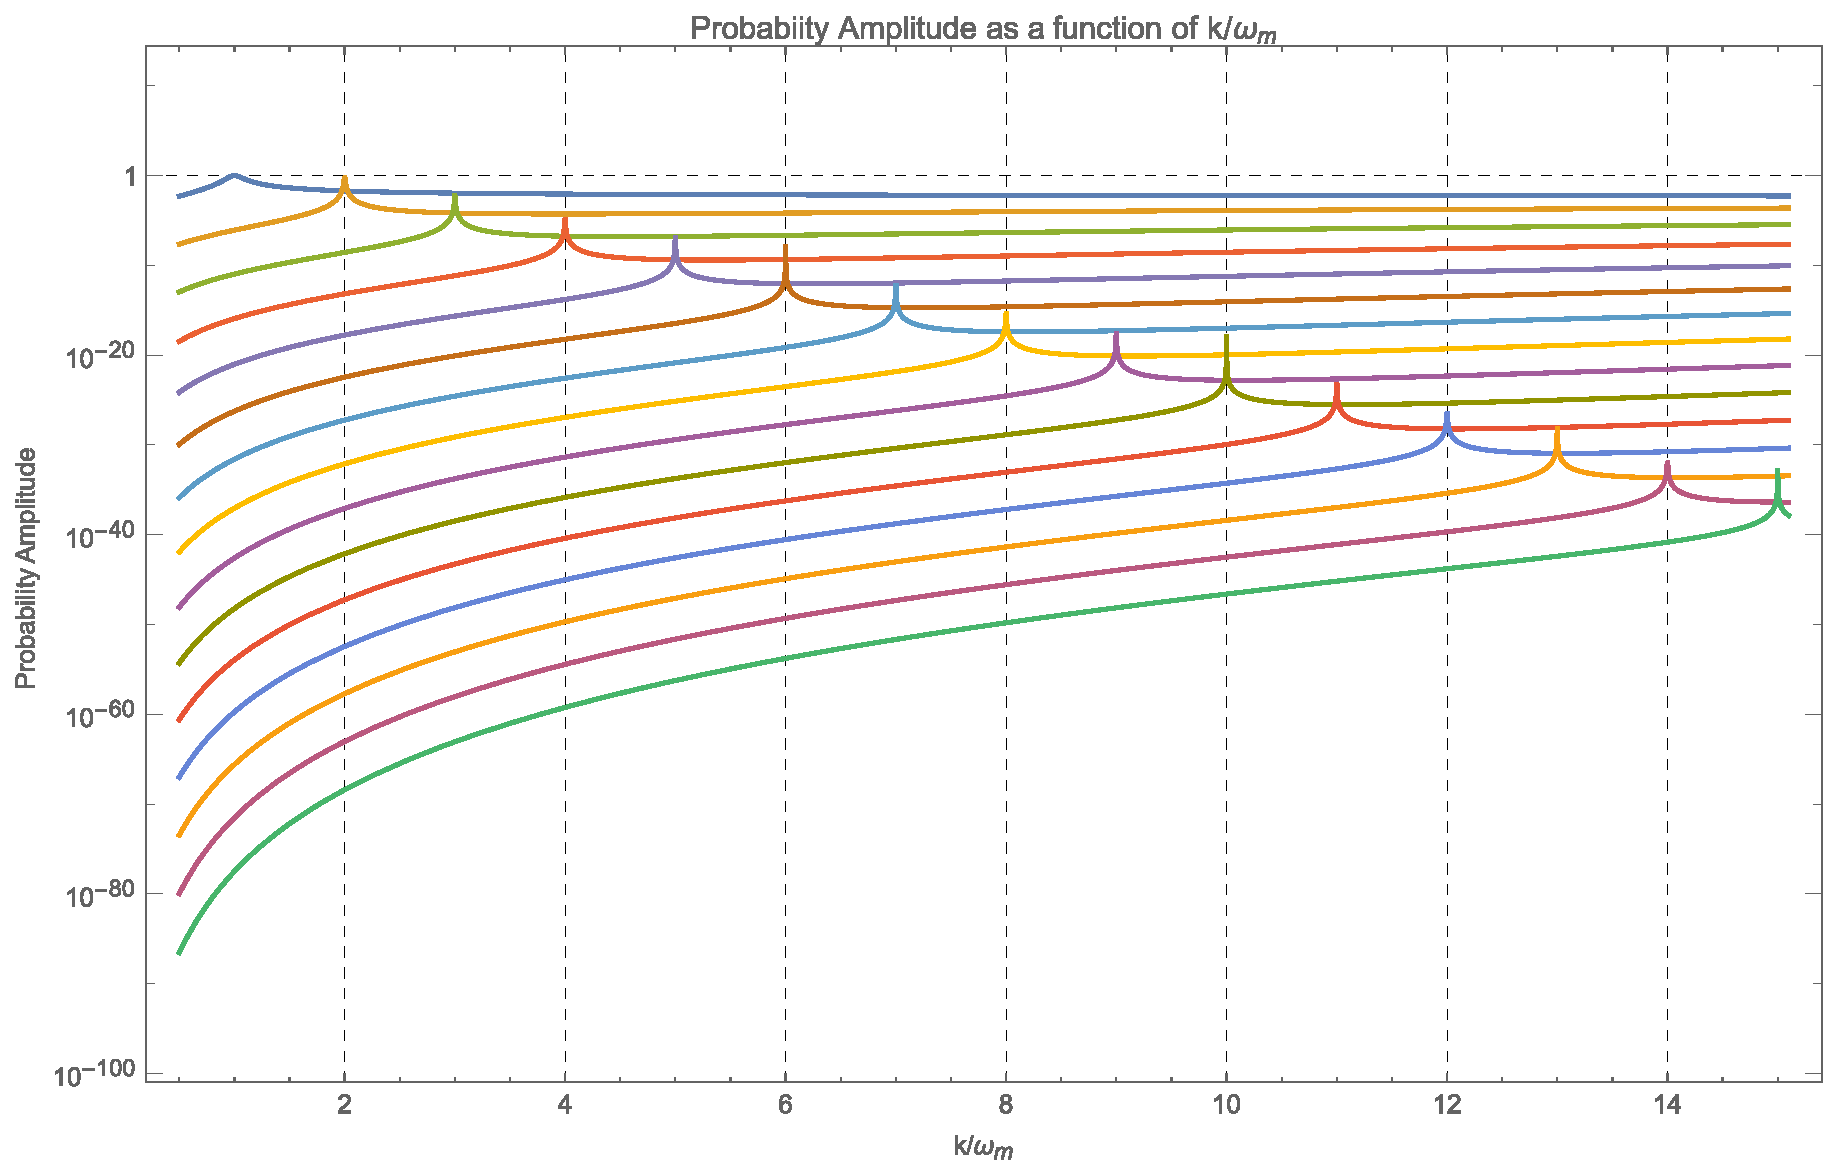
\includegraphics[width=\textwidth]{chapters/assets/rabi/stimulated-probability-apmlitude-vs-k-Jacobi-Anger.pdf}
%     \caption{Probability amplitude as a function of $k/\omega_{\mathrm m}$ for each term in Jacobi-Anger expansion, with parameters $\lambda_1=0.1$,$\theta_{\mathrm m}=\pi/5$.}
%     \label{chap:matter-sec:single-revisted-fig:prob-amp-jacobi-anger}
% \end{figure}


% \begin{figure}[!htbp]
%     \centering
%     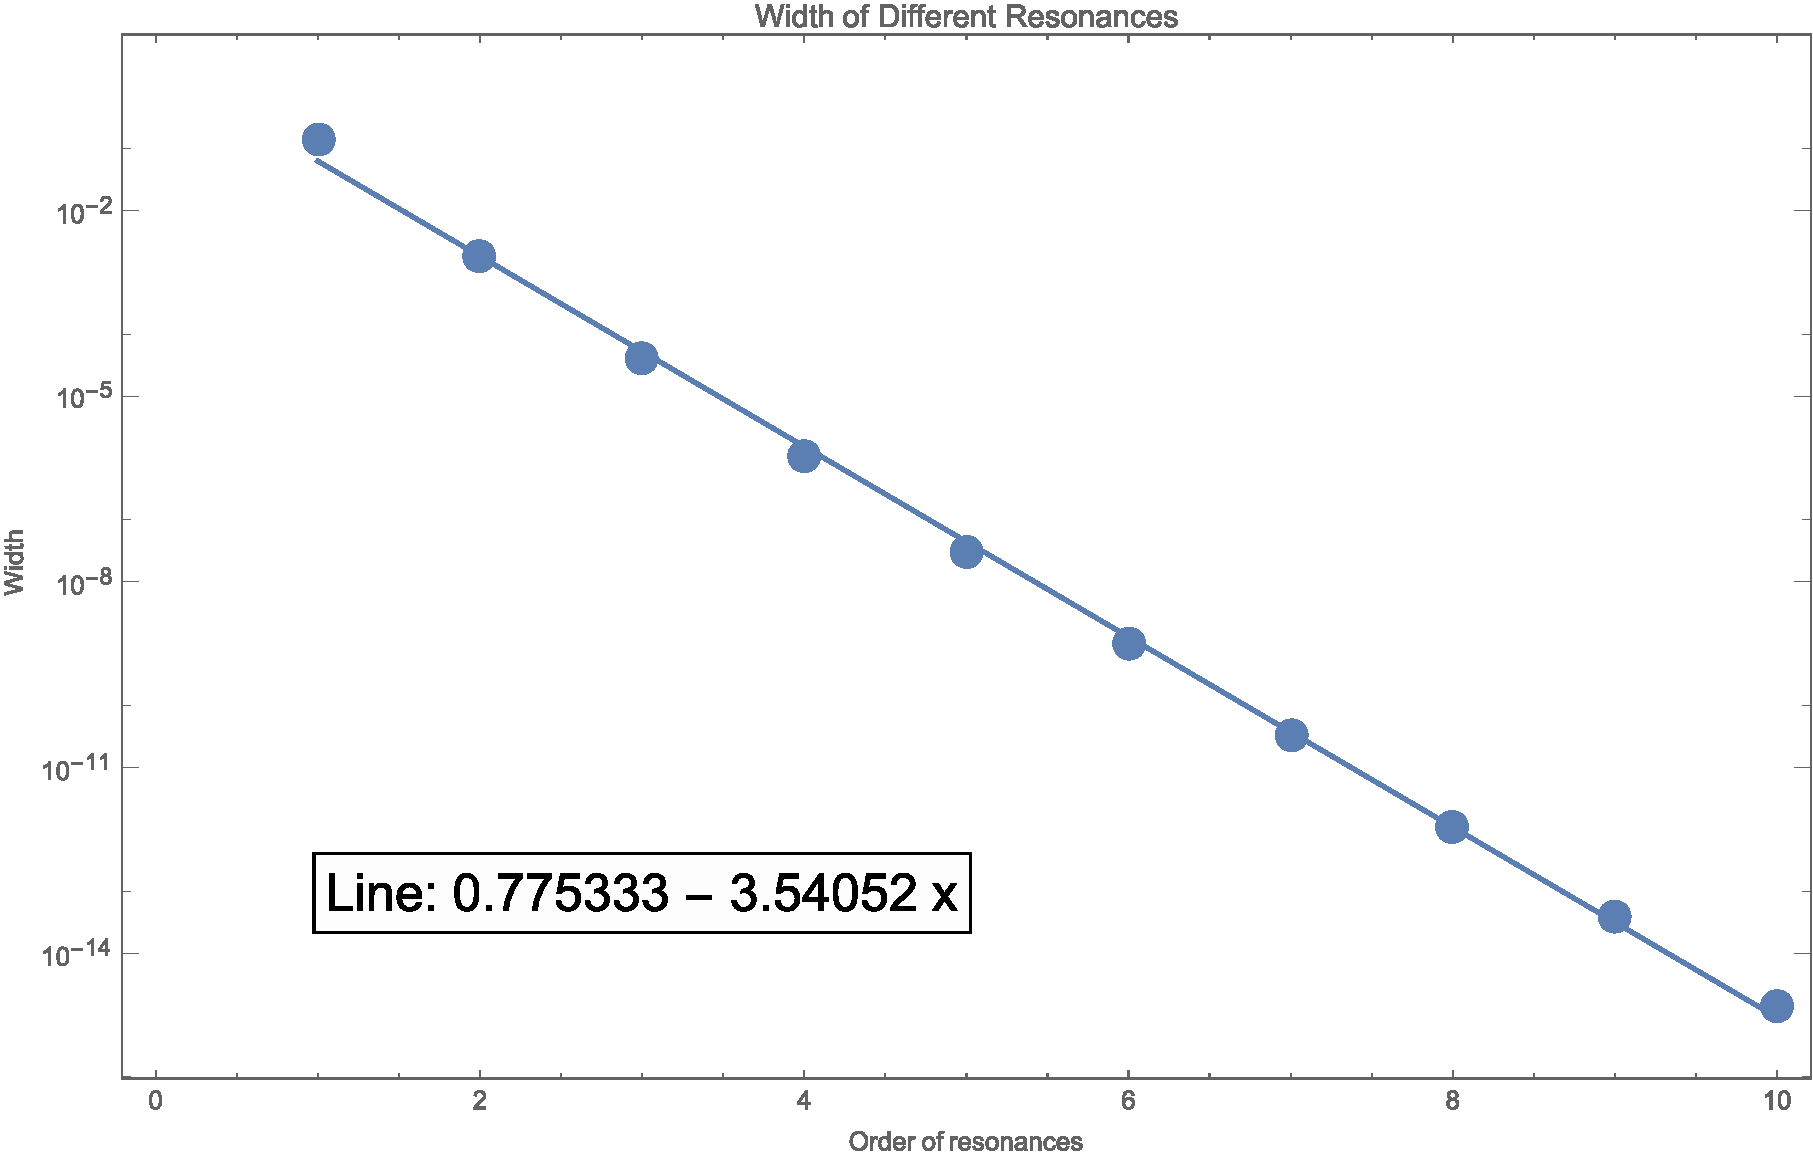
\includegraphics[width=\textwidth]{chapters/assets/rabi/stimulated-probability-apmlitude-vs-k-resonance-width.pdf}
%     \caption{Resonance width as a function of mode order for each term in Jacobi-Anger expansion, with parameters $\lambda_1=0.1$,$\theta_{\mathrm m}=\pi/5$.}
%     \label{chap:matter-sec:single-revisted-fig:resonance-width-jacobi-anger-exp}
% \end{figure}



% \begin{figure}[!htbp]
%     \centering
%     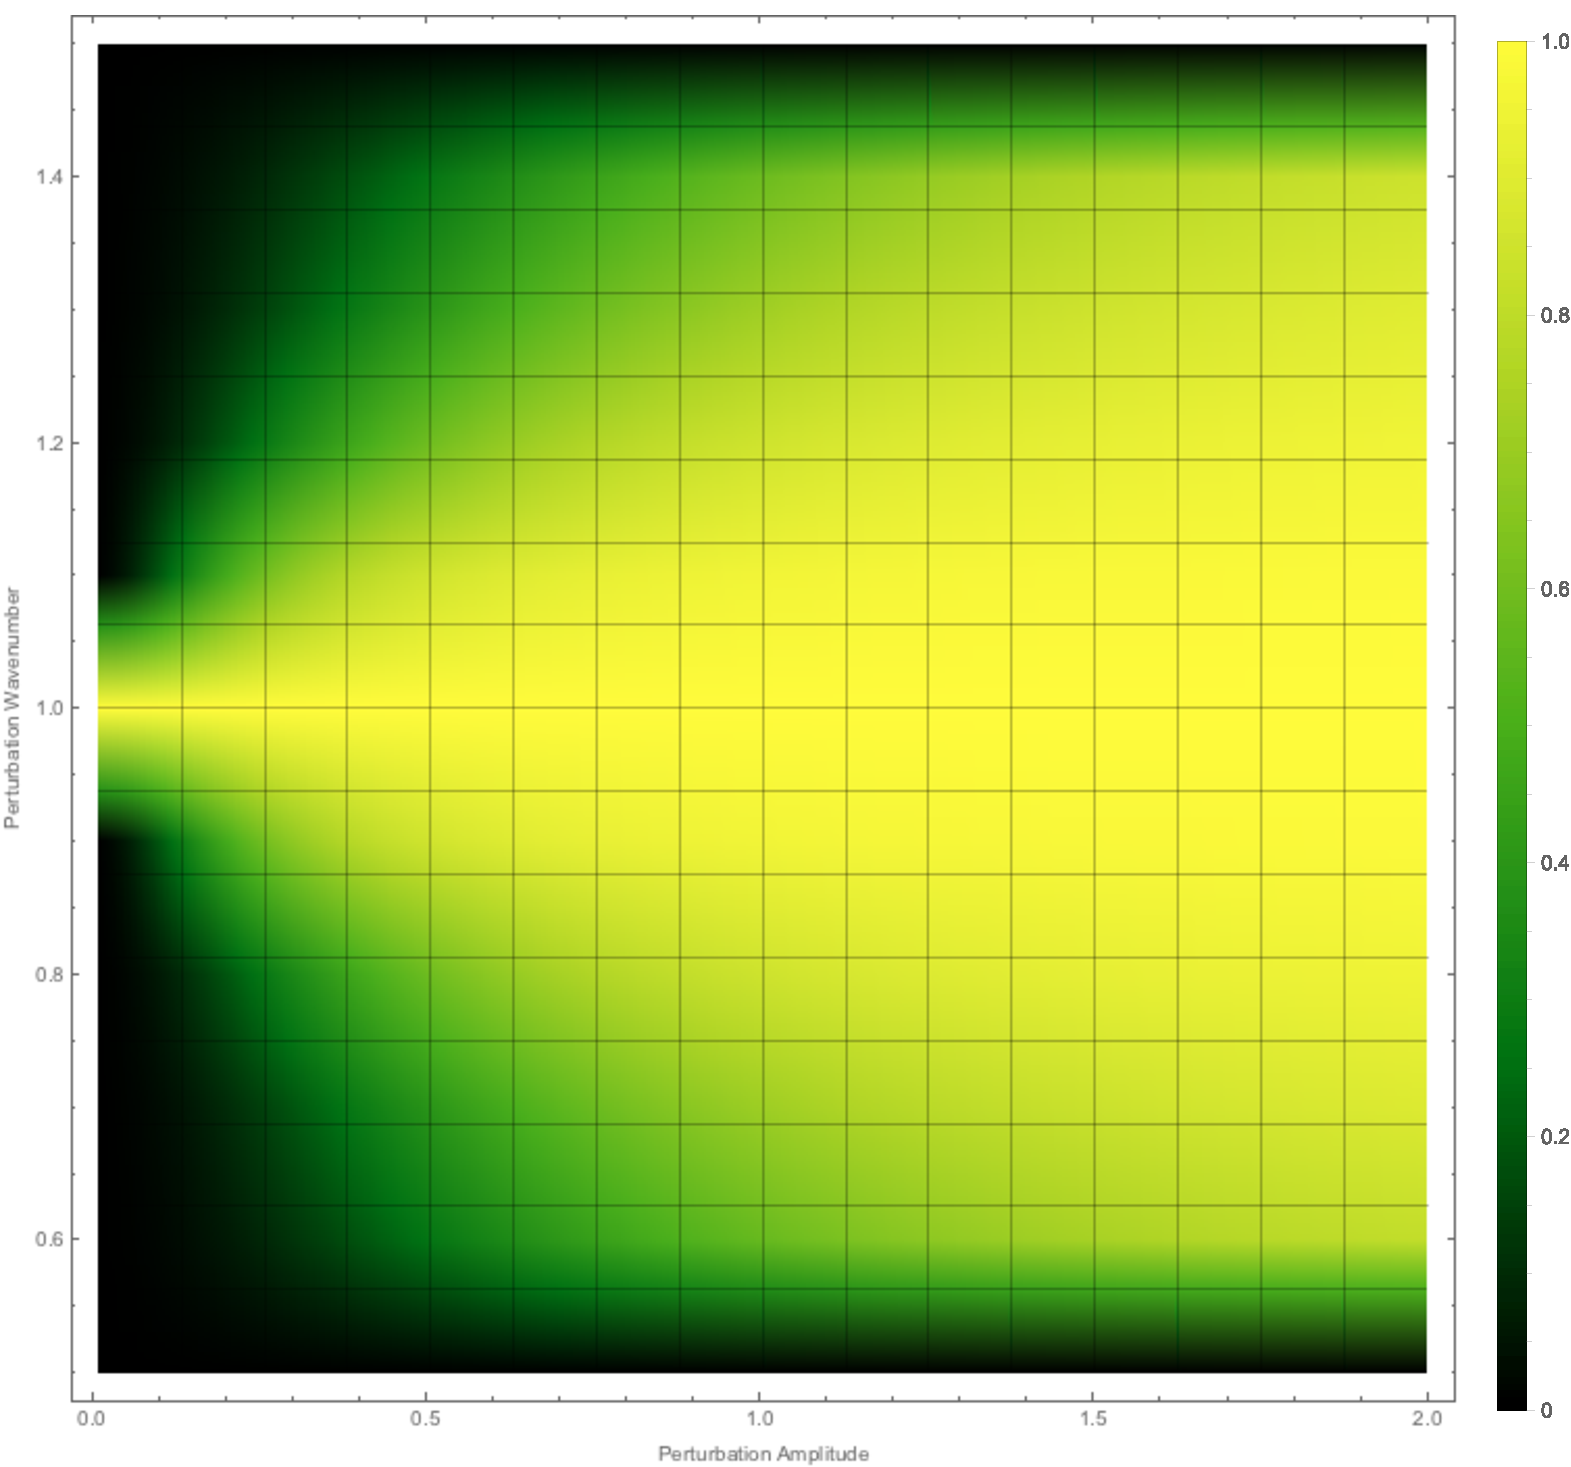
\includegraphics[width=\textwidth]{chapters/assets/rabi/pltPertAmpPertWaveNumTransitionAmp}
%     \caption{Transition probability amplitude at different perturbation amplitude and perturbation wavenumber. Larger amplitudes corresponds to larger resonance width, as another confirmation to Fig.~\ref{chap:matter-sec:single-revisted-fig:resonance-width-jacobi-anger-exp}.}
%     \label{chap:matter-sec:single-revisted-fig:resonance-width-heatmap}
% \end{figure}



\subsection{\label{chap:matter-subsec:multi-frequency-revisited}Multi-frequency Matter Profile Revisited}


For multi-frequency matter profiles $\delta \lambda(r) = \sum_n \lambda_n \sin (k_n r)$, the derivation is the same as the derivation for single frequency matter profiles but with more tedious math. The Hamiltonian in Rabi basis is
\begin{equation}
    \mathsf H^{(\RR)} = -\frac{\omega_\mm}{2}\sigma_3 + \begin{pmatrix}
        0 & h\\
        h^{*} & 0
        \end{pmatrix},
\end{equation}
where the off diagonal element $h$ is
\begin{equation}
    h = \frac{\sin 2\theta_\mm}{2} \sum_a \lambda_a \sin (k_a x) \prod_{a} \sum_{n=-\infty}^{\infty} (-i)^n J_n (z_{k_a}) e^{i n(k_a x) }
\end{equation}

% To demonstrate the procedure of Jacobi-Anger expansion as well as the technique
% to decompose the problem into simple Rabi oscillations, I adopt the two frequencies
% matter density scenario. The Hamiltonian is described in Eqn.~\ref{eq-hamiltonian-bg-matter-basis-multi-frequency}. The term $h$ becomes
% \begin{equation}
%     h = \frac{\sin 2\theta_\mm}{2} \sum_{a = 1}^2 \lambda_a \sin (k_a r) \prod_{a=1}^2 \sum_{n=-\infty}^{\infty} (-\ri)^n J_n ( \lambda_a \cos 2\theta_\mm/{k_a} ) e^{\ri n k_a r }.
%     \label{chap:matter-subsec:multi-frequency-revisited-eqn:rabi-hamil-off}
% \end{equation}
% The summations and products can be rewritten using the trick,
% \begin{equation}
%     \sum_n a_n \sum_\mm b_\mm  = \sum_{N = -\infty}^{\infty} \sum_{m+n=N} a_n b_\mm = \sum_{N=-\infty}^\infty \sum_{n=-\infty}^{N} a_n b_{N-n}.
%   \label{chap:matter-subsec:multi-frequency-revisited-eqn:multiplication-summation-rule}
% \end{equation}
% For further simplifications of the problem, I follow a rule to sum over a line $m+n=N$ then sum over $N$, which is illustrated in Fig.~\ref{chap:matter-sec:jacobi-subsec:multi-matter-freq-fig:summation-algebra}.
% \begin{figure}[!htbp]
%     \centering
%     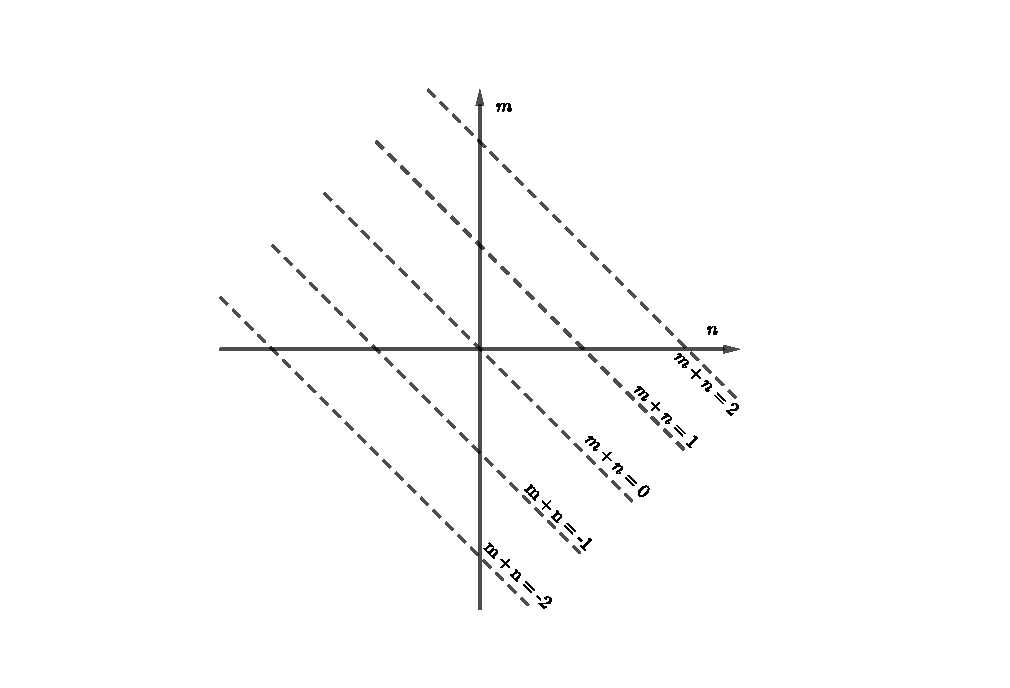
\includegraphics[width=\textwidth]{chapters/assets/rabi/summation-algebra}
%     \caption{Rewrite multiplication of summations into summations only. The horizontal axis is for the summation index $n$ and the vertical axis is for the summation index $m$. The dashed lines are the lines of equal $m+n$.}
%     \label{chap:matter-sec:jacobi-subsec:multi-matter-freq-fig:summation-algebra}
% \end{figure}
% Eqn.~\ref{chap:matter-subsec:multi-frequency-revisited-eqn:rabi-hamil-off} becomes
% \begin{align}
%    h =& \frac{\sin 2\theta_\mm}{2} \sum_{a = 1}^2 \lambda_a \sin (k_a r)  \nonumber\\
%    &\sum_{N=-\infty}^{\infty} \sum_{n=-\infty}^{N} (-\ri)^n J_n ( \lambda_1 \cos 2\theta_\mm / k_1) e^{i n k_1 r } (-\ri)^{N-n} J_{N-n}( \lambda_2\cos 2\theta_\mm /k_2) e^{\ri (N-n)(k_2 r)} \nonumber\\
%    =&\frac{\sin 2\theta_\mm}{2} \sum_{a = 1}^2 \lambda_a \sin (k_a r )  \nonumber\\
%    &\sum_{N=-\infty}^{\infty} \sum_{n=-\infty}^{N} (-\ri)^N J_{n}( \lambda_1\cos 2\theta_\mm / k_1) J_{N-n}(  \lambda_2 \cos 2\theta_\mm /k_2 ) e^{\ri n ((k_1-k_2)r ) + \ri N (k_2 r)}
%    \label{chap:matter-sec:jacobi-subsec:multi-matter-freq-eqn:stimulated-multi-freq-hamiltonian-12-element}
% \end{align}
% I can also rewrite $\sum_{a = 1}^2 \lambda_a \sin (k_a r)$,
% \begin{align}
%    &\lambda_1 \sin(k_1 r ) + \lambda_2 \sin(k_2 r) \nonumber\\
%    = & \frac{\lambda_1}{2 \ri}\left( e^{\ri(k_1 r)} +  e^{-\ri(k_1 r)} \right) + \frac{\lambda_2}{2\ri} \left( e^{\ri(k_2 r)} +  e^{-\ri(k_2 r)} \right).
% \end{align}
% Using the relation Eqn.~\ref{eqn:bessel-function-sum-property}, I can combine the terms and simplify $h$ to
% \begin{equation}
% \end{equation}

Using the relations of Bessel functions in Eqn.~\ref{eqn:bessel-function-sum-property}, I can decompose $h$ into two terms
\begin{align}
    h =& -\sum_{n_1 = -\infty}^\infty \sum_{n_2 = -\infty}^\infty  (-\ri)^{ \sum_a n_a} \frac{\tan 2\theta_\mm}{2} \sum_a n_a k_a \\
    & J_{n_1} ( \lambda_1 \cos 2\theta_\mm/k_1)  J_{n_2} ( \lambda_2 \cos 2\theta_\mm/k_2)  e^{  \ri \sum_a n_a k_a r } .
\end{align}

The arguments that I applied to single frequency matter profile are still valid for multi-frequency matter profiles. For completeness of this section, I will present one example of multi-frequency matter profile. One of the multi-frequency matter profiles that has been well studied is the castle wall matter profile. I can decompose the periodic castle wall matter profile into many Fourier modes and study the interference effect. The potential shown in Fig.~\ref{fig-castlewall-profile-illustration} is defined as,
\begin{equation}
    \lambda(r) = \begin{cases}
\Lambda_1, &\quad -\frac{X_1}{2}+nX\le r\le \frac{X_1}{2}+nX \\
\Lambda_2, &\quad \frac{X_1}{2}+nX\le r\le \frac{X_1}{2}+\frac{X_2}{2} +nX
\end{cases}
\label{eq-castle-wall-potential}
\end{equation}
where $X_1$ and $X_2$ are the two periods of the matter profile or potential, $X=X_1+X_2$, and $n$ is integer. The parametric resonance condition derived by E. Akhmedov~\cite{Akhmedov2000} is,
\begin{equation}
    \frac{\tan (\omega_{\mathrm m1}X_1/2)}{\tan (\omega_{\mathrm m2}X_2/2)} = - \frac{\cos 2\theta_{\mathrm m2}}{\cos 2\theta_{\mathrm m1}},
    \label{eq-akhmedov-resonance-condition-castle-wall}
\end{equation}
where $\omega_{\mathrm{m}i}$ and $\theta_{\mathrm{m}i}$ are the energy difference and mixing angle for potential $\Lambda_1$ and $\Lambda_2$ respectively.

Even though this castle wall problem is analytically solved, the resonance condition Eqn.~(\ref{eq-akhmedov-resonance-condition-castle-wall}) itself is not transparent. In this subsection, we show that such a system is closed related to Rabi oscillations. For illustration purpose, we set the profile to be equal period for the two densities so that $X_1=X_2\equiv X/2$. To show that the neutrino flavor conversions in this castle wall matter profiles is related to Rabi oscillation, we decompose the profile using Fourier series,
\begin{equation}
\lambda(r) = \lambda_0 + \sum_{n=1}^{\infty} \lambda_n \cos\left( k_n  r \right),
\label{eq-castle-wall-fourier-expanded}
\end{equation}
where
\begin{align*}
\lambda_0 &= (\Lambda_1 + \Lambda_2)/2, \\
\lambda_n & = \frac{2}{(2n-1)\pi}  (-1)^n  \left( \Lambda_1 -  \Lambda_2 \right),\\
k_n &= (2n-1)k_0, \\
k_0 &= 2\pi/X.
\end{align*}
The decomposition is visualized in Fig.~\ref{app-chap:convention-sec:fourier-series-eqn:parametric-resonance-castle-wall-fourier-coeff-even}.

To calculate the transitions between two mass states of background matter potential $\lambda_0$, we use the background matter basis with respect to $\lambda_0$, in which the transition is zero when varying matter profile vanishes. The Hamiltonian
\begin{equation}
\mathsf H^{(\mathrm m)} = - \frac{1}{2}\omega_{\mathrm m} \sigma_3  + \frac{1}{2} \sum_{n=1}^{\infty} \lambda_n \cos 2\theta_{\mathrm m} \cos\left( k_n  r \right)  \sigma_3 - \frac{1}{2} \sum_{n=1}^{\infty} \lambda_n \sin 2\theta_{\mathrm m}  \cos\left( k_n r \right) \sigma_1,
\label{castle-wall-decomposed-hamiltonian}
\end{equation}
determines the transitions between the two background matter states.


\begin{figure}[!htbp]
    \centering
    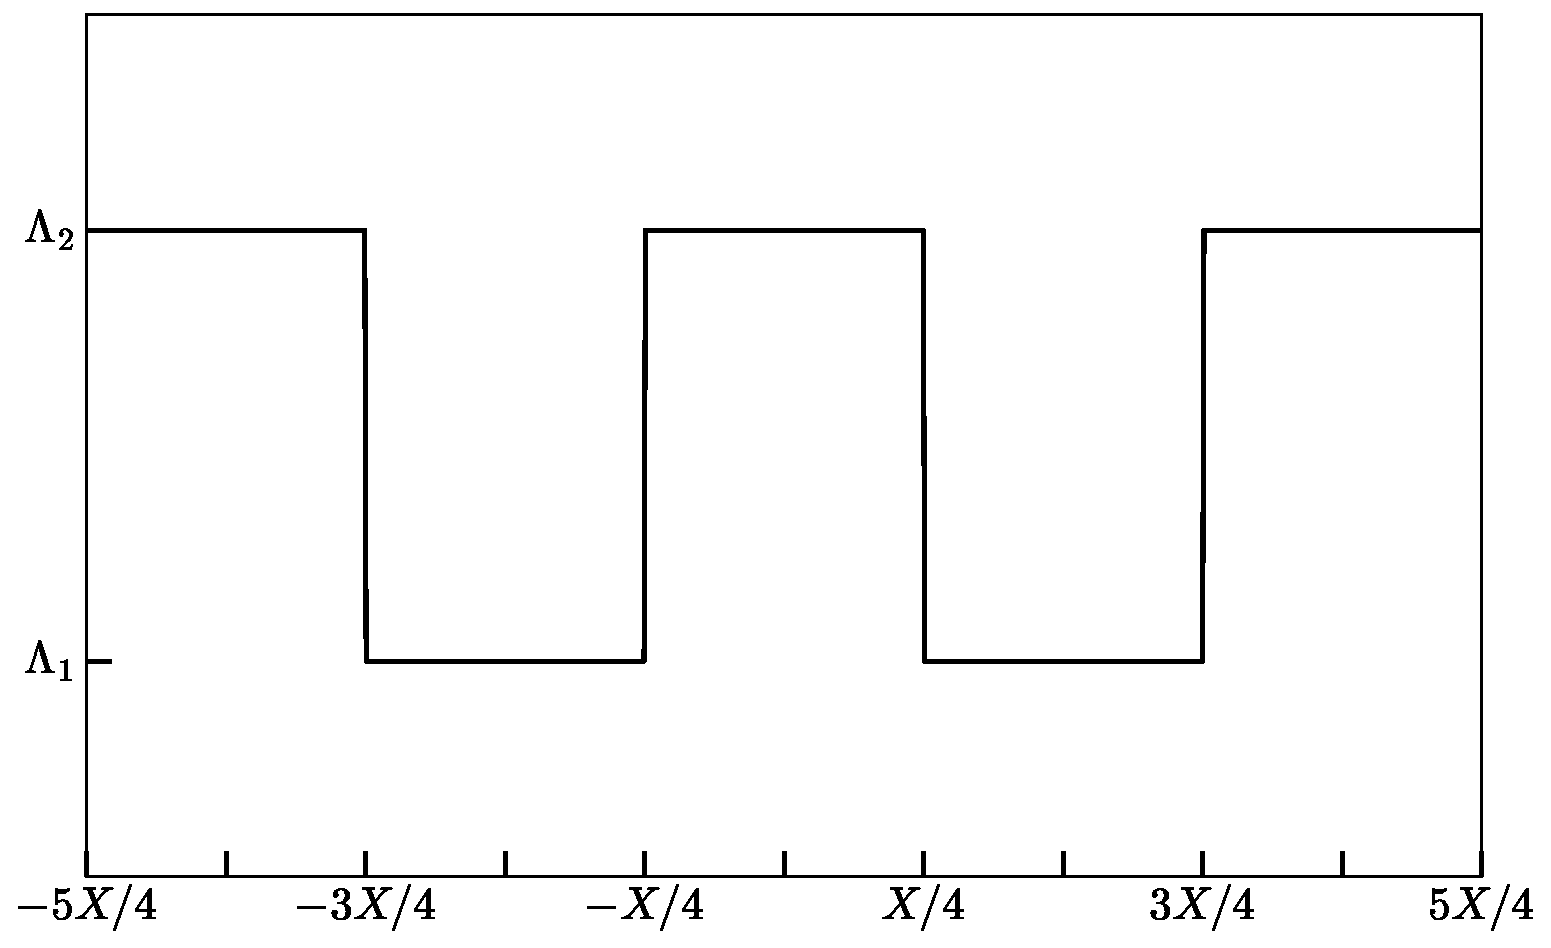
\includegraphics[width=\columnwidth]{chapters/assets/rabi/castlewall-profile}
    \caption{The castle wall matter potential profile with $X_1=X_2=X/2$.}
    \label{fig-castlewall-profile-illustration}
\end{figure}



% \begin{figure}[!htbp]
%     \centering
%     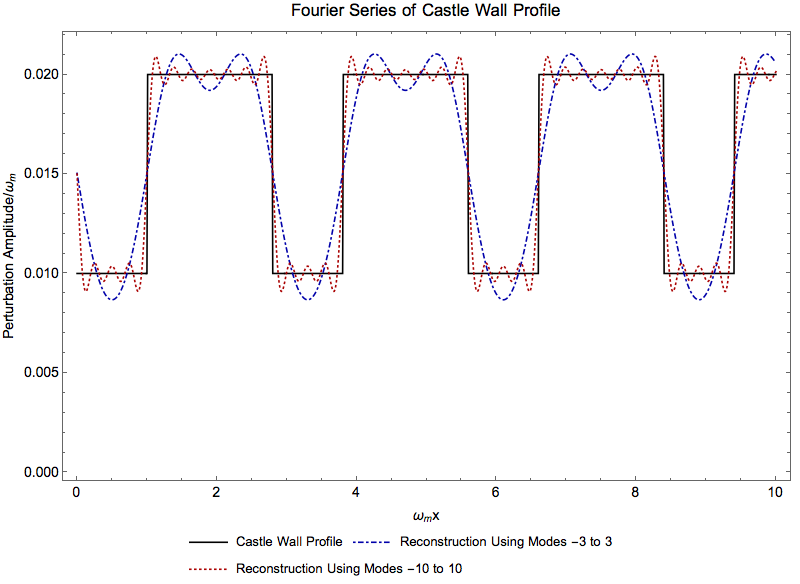
\includegraphics[width=\textwidth]{chapters/assets/rabi/reconstruction-of-castle-wall-0point01-0point02-1-1point8}
%     \caption{Decomposition of castle wall density profile using Fourier modes.}
%     \label{chap:matter-sec:castlewall-fig:decompose-castlewall-fourier}
% \end{figure}


\begin{figure}[!htbp]
        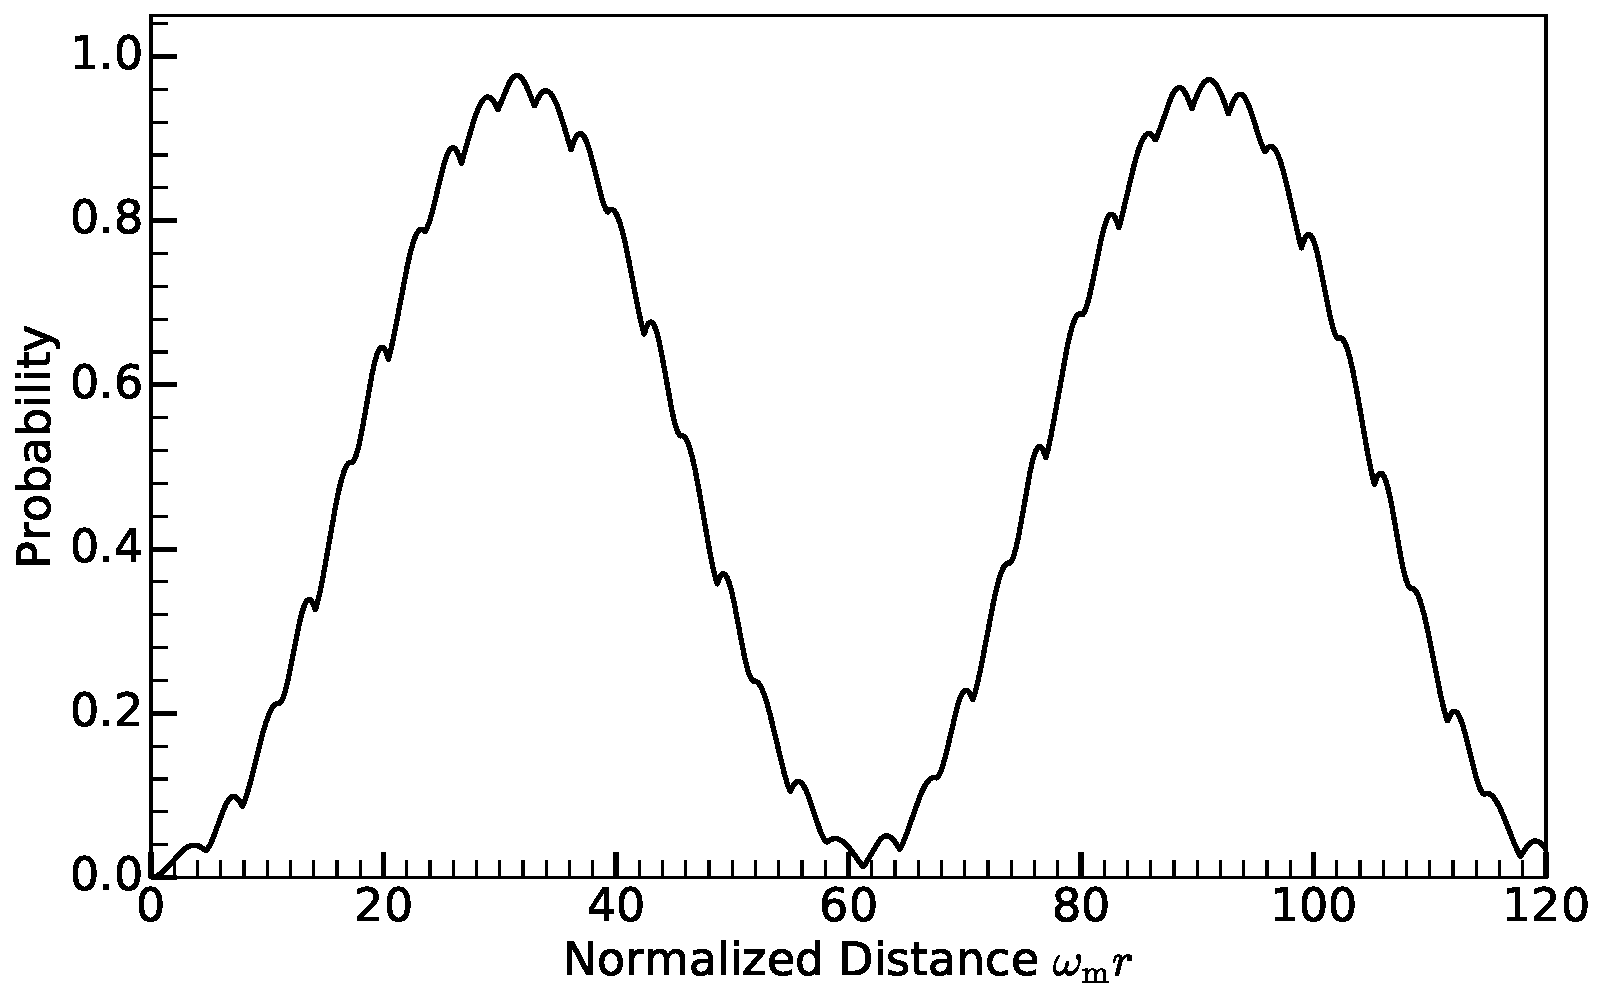
\includegraphics[width=\columnwidth]{chapters/assets/rabi/castle-wall-1}%
    \caption{Transition probabilities for castle wall matter profile calculated numerically for $\Lambda_2-\Lambda_1=0.4 \Lambda_0$. During the calculation, the energy of neutrinos is $10\,\mathrm{MeV}$, mass-squared difference is $\delta m^2=2.6\times 10^{-3}\,\mathrm{eV^2}$, and the vacuum mixing angle chosen so that $\sin^2(2\theta_\vv)=0.093$. The background potential $\Lambda_0$ is chosen so that it's half the MSW resonance potential, $\Lambda_0 = \frac{1}{2}\lambda_{\mathrm{MSW}}=\frac{1}{2}\omega_{\mathrm{v}}\cos 2\theta_{\mathrm v}$, and the base frequency is set to $k_0 = 2\pi/X = \omega_{\mathrm{m}}$.
                 }
    \label{fig-akhmedovOscPlt}
\end{figure}


The base frequency $k_0$ which is determined by the total period $X$ can be arbitrary. In this example, we choose a $X$ so that the base frequency $k_0$ matches the energy gap $\omega_{\mathrm{m}}$. Even though multiple perturbation frequencies show up in Eqn.~(\ref{castle-wall-decomposed-hamiltonian}), we identify that only the first frequency $n=1$ is the resonance frequency since we are using $k_0=\omega_{\mathrm{m}}$. As an approximation, we drop all other frequencies $n>2$ regarding the fact that they are far from resonance. Thus, similar to single frequency matter profile, the varying $\sigma_3$ terms have limited effects on the transition probabilities in our case, which leads to
\begin{align*}
    H^{(\mathrm m)} \to & - \frac{1}{2}\omega_{\mathrm m} \sigma_3  - \frac{1}{2} \sum_{n=1}^2\lambda_n \sin 2\theta_{\mathrm m}  \cos\left( k_n r \right) \sigma_1\\
    \to & - \frac{1}{2}\omega_{\mathrm m} \sigma_3  - \frac{1}{2} \sum_{n=1}^2 A_n \cos ( k_n r) \sigma_1 \\
    & + \frac{1}{2} \sum_{n=1}^2A_n \sin(k_n r) \sigma_2,
\end{align*}
where
\begin{equation*}
A_n = \frac{\lambda_n \sin 2\theta_{\mathrm m} }{2} .
\end{equation*}
The relative detuning is $0$ if we have only the first mode. However, it becomes
\begin{equation}
\RD_1'= \frac{A_2^2}{2\lvert A_1 (\omega_{\mathrm m} - k_2) \rvert},
\end{equation}
if we include the second frequency $k_2$. One feature of this Fourier series expanded matter profile Eqn.~(\ref{eq-castle-wall-fourier-expanded}) is that the width of each frequency decreases as the order $n$ increases while the detuning of each frequency increases. We calculate the relative detuning for each frequency
\begin{equation}
\RD_n = \frac{\lvert k_n -\omega_{\mathrm m} \rvert}{ \lvert \lambda_n  \sin 2\theta_{\mathrm m}/2 \rvert } = \frac{2(n-1)(2n-1)\pi \omega_{\mathrm m}}{(\Lambda_2 - \Lambda_1)\sin 2\theta_{\mathrm m}}
\end{equation}
which is quadratic in $n$ and inversely proportional to $\Lambda_2-\Lambda_1$. We find that all higher frequencies $k_n$ for $n>2$ have very large relative detunings. The neutrino transition probability between the two matter states is shown in Fig.~\ref{fig-akhmedovOscPlt}, where we find the system has almost full transition.

A more rigorous treatment is to use Jacobi-Anger expansion and find the Rabi modes, where we find that the mode that corresponds to single frequency $k_1$ dominates and all other modes have little destruction effect on it. Quantitatively, higher orders leads to smaller width $B_{\{n_i\}}$ yet larger detuning $\sum_{n} nk_n-\omega_{\mathrm m}$, which renders a smaller effect on the resonance mode $\{1,0\}$, since the effect is evaluated as Eqn.~(\ref{chap:matter-eq:relative-detuning-changed}).
Table~\ref{tab-q-values-each-mode} lists the first few smallest relative detunings of Fig.~\ref{fig-akhmedovOscPlt}. The second column is the relative detuning of the corresponding mode, while the third column is the relative detuning of mode $\{1,0\}$ with the energy gap shift effect of the corresponding mode.



% Find the data in MMA file `akhmedov-parametric-resonance.nb`
% {0., 6129.81, 20432.7, 42908.7}
% {0., 5.99981, 19.9994, 41.9987}

\begin{table}
\centering

% \begin{ruledtabular}
\begin{tabular}{lll}
\hline
 $\{n_1,n_2\}$ &  $\RD$ & $\RD'_{\{1,0\}}$   \\
\hline
 $\{1,0\}$ & $0$ &  - \\
 $\{-1,0\}$ & $48$ &  $1.0\times 10^{-2}$ \\
 $\{0,1\}$ & $1.5\times 10^2$ &  $1.1\times 10^{-3}$  \\
 $\{2,0\}$ & $2.4\times 10^{2}$ & $2.0\times 10^{-4}$ \\
 \hline
\end{tabular}
% \end{ruledtabular}
\caption{\label{tab-q-values-each-mode}Relative detuning of each frequency.}
\end{table}






\section{\label{conclusions}Conclusions}



The solar neutrinos behave very differently from lab experiments since the Sun provides a high matter density lab which can not be built on the Earth. What's even more exotic, in a supernova explosion, $10^{58}$ neutrinos are released from the proto-neutron star, which is of radius $10\mathrm{km}$, in a few seconds. The huge number density of neutrinos and large density of matter both change the neutrino oscillations dramatically. The matter effect in supernova is also much more complicated than MSW for solar neutrinos since the rich distribution of matter density and high speed motion. In addition to matter effect, neutrino neutrino interaction will be very efficient because of the high neutrino number density.

Apart from the emission of neutrinos from nuclear reactions of electron capture and positron emission in the solar interior, supernova environment also gives rise to Bremsstrahlung pair neutrino production, electron-positron neutrino pair production, which brings all three flavors and also anti-neutrinos into the spectra. However, even the with the presence of intensive interaction between neutrinos and the leptons and hardrons, which thermalize the neutrinos in the supernova core, the neutrino spectrum escaping from the supernova core is not completely Fermi-Dirac distribution. Nonetheless, it is possible to parametrize it using nominal Fermi-Dirac distribution,\cite{ysuzuki2004}
\begin{equation}
f(E)\propto \frac{E^2}{1+\exp ( E/kT - \mu )}.
\end{equation}
Some numerical results show that there is a deviation from this Fermi-Dirac distribution~\cite{Totani1998,Keil2003}. Meanwhile, Keil Mathias and Georg Raffelt showed that it is good enough to approximate the neutrino spectrum from supernova in Monte Carlo simulations using the so called "alpha fit",
\begin{equation}
f(E)\propto E^\alpha \exp\left( -(\alpha+1)\frac{E}{\langle E\rangle} \right),
\end{equation}
where $\langle E\rangle$ is the average energy, or the first moment of energy. The values from Monte Carlo simulations falls into the range $\alpha = 2.5\sim 5$,
which clearly shows the spectra are pinched. It's a hint that the detection of deviation from nominal Fermi-Dirac distribution will show evidence of core-collapse information.


% \begin{figure}
% \centering
% 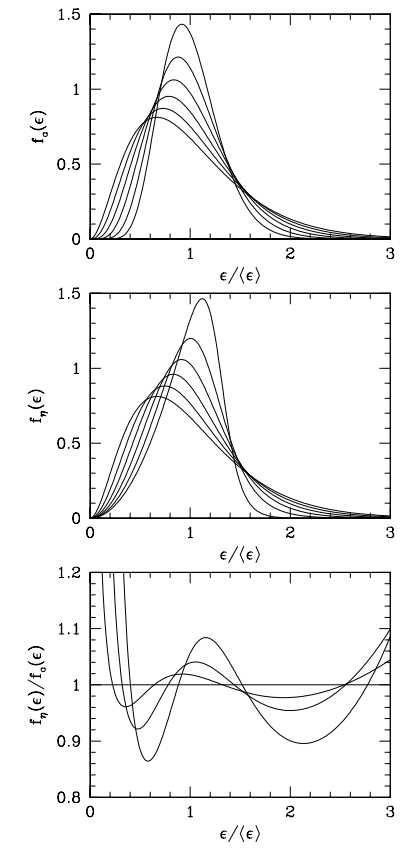
\includegraphics[width=\columnwidth]{chapters/assets/solar/neutrino_spectra_sn_simulations.png}
% \caption{Alpha fit and nominal Fermi-Dirac fit comparison. The top panel is alpha fit results while the middle panel is from nominal Fermi-Dirac distribution fit. The broadest curve are for $\alpha=2$. The width $w=\sqrt{\langle E^2 \rangle - \langle E\rangle^2}$ decrease 10\% for each curve. The bottom panel is the ratio of the two fit functions.}
% \label{fig:neutrino_spectra_sn_simulations}
% \end{figure}


Even though we understand solar neutrinos well, the neutrino oscillations of supernova explosions are not so to our complete knowledge. The flavor content is subject to the solution to the neutrino oscillations. Phenomena such as spectral split due to neutrino-neutrino interaction and matter effect reshape the neutrino spectra significantly. That being said, more research on supernova neutrinos, especially supernova neutrino oscillations is critical to understand supernova explosion mechanisms, as well as future observation of supernova neutrino data.


In conclusion, we have provided an interpretation for neutrino flavor conversion in fluctuating matter with the help of Rabi oscillations. The work provided two different points of view that is related to Rabi oscillations.

The first point of view was to interpret the neutrino flavor conversions in background matter basis. In this basis, matter density fluctuations will introduced a fluctuation part to the diagonal elements of the Hamiltonian, which means that the energy gap is fluctuating if we draw analogy between this Hamiltonian and the Hamiltonian of Rabi oscillations. For neutrino flavor conversions in a single frequency matter profile, the neutrino flavor oscillations becomes large when the matter fluctuation frequency is close to the energy gap, which is the resonance condition. We anticipated that the fluctuations of energy gap have limited effects on neutrino flavor conversions under this resonance condition. Thus the matter fluctuation only works as a pure flipping field that converts neutrinos from one flavor to another.

As we added more frequencies of matter density fluctuations, the neutrino flavor conversions becomes nontrivial due to the interferences between the difference matter profile frequencies. To quantify the interference between different Rabi oscillation modes, we defined relative detuning which describes how off-resonance a Rabi oscillation is. In the case of single frequency Rabi oscillations, the relative detuning becomes $0$ under the resonance condition. As a second frequency is added to the oscillations, the energy gap is shifted due to this new frequency. A measure of the interference effect is to consider the relative detuning of the first frequency which is at resonance, under the shifted energy gap. Numerical results verified this conjecture. With the interference mechanism, we revisit the single frequency matter profile neutrino oscillations.

Another view is to switch to a basis where the neutrino oscillations Hamiltonian is decomposed into infinite Rabi oscillations. Equivalently speaking, the oscillations are consequences of superposition of Rabi oscillations, which we call modes of oscillations. This view was applied to emphasis the approximations that the change of energy gap due to matter fluctuation can be neglected under resonance condition in the previous background matter basis.











% \section{\label{acknowledgement}Acknowledgement}

% The first author would like to thank J. Kneller and K. Patton for their help during this research. This research is supported by DOE EPSCoR grant \#DE-SC0008142.
